% Copyright 2015-2017 Dan Foreman-Mackey and the co-authors listed below.

\documentclass[manuscript, letterpaper]{aastex6}

\pdfoutput=1

%%% This file is generated by the Makefile.
\newcommand{\githash}{108ca20}\newcommand{\gitdate}{2016-09-06}\newcommand{\gitauthor}{Eric Agol}
\newcommand{\exampleindata}{200}
\newcommand{\exampleinwalkers}{32}
\newcommand{\exampleinburn}{500}
\newcommand{\exampleinsteps}{2000}
\newcommand{\exampleineff}{1737}
\newcommand{\exampleiindata}{100}
\newcommand{\exampleiinwalkers}{32}
\newcommand{\exampleiinburn}{500}
\newcommand{\exampleiinsteps}{2000}
\newcommand{\exampleiineff}{1134}
\newcommand{\exampleiiindata}{6950}
\newcommand{\exampleiiinwalkers}{32}
\newcommand{\exampleiiinburn}{500}
\newcommand{\exampleiiinsteps}{5000}
\newcommand{\exampleiiineff}{2900}
\newcommand{\exampleivndata}{1440}
\newcommand{\exampleivnwalkers}{32}
\newcommand{\exampleivnburn}{5000}
\newcommand{\exampleivnsteps}{15000}
\newcommand{\exampleivneff}{1443}
\newcommand{\examplevndata}{1000}
\newcommand{\examplevnwalkers}{32}
\newcommand{\examplevnburn}{10000}
\newcommand{\examplevnsteps}{30000}
\newcommand{\examplevneff}{1490}

% Automatically generated
\newcommand{\rotationperiod}{\ensuremath{{3.79 \pm 0.15}}}


\usepackage{microtype}
\usepackage{url}
\usepackage{amsmath}
\usepackage{amssymb}
\usepackage{natbib}
\usepackage{multirow}
\bibliographystyle{aasjournal}

% ----------------------------------- %
% start of AASTeX mods by DWH and DFM %
% ----------------------------------- %

% Matrix fix:
% http://tex.stackexchange.com/questions/317824/letter-c-appearing-inside-pmatrix-environment-with-aastex
\makeatletter
\def\env@matrix{\hskip -\arraycolsep % taken from amsmath.sty lines 895ff
  \let\@ifnextchar\new@ifnextchar
  \array{*{\c@MaxMatrixCols}c}}
\makeatother

% Column spacing in matrix
% http://tex.stackexchange.com/questions/275725/adjusting-separation-between-matrix-entries
\setlength\arraycolsep{25pt}

\setlength{\voffset}{0in}
\setlength{\hoffset}{0in}
\setlength{\textwidth}{6in}
\setlength{\textheight}{9in}
\setlength{\headheight}{0ex}
\setlength{\headsep}{\baselinestretch\baselineskip} % this is 2 lines in ``manuscript''
\setlength{\footnotesep}{0in}
\setlength{\topmargin}{-\headsep}
\setlength{\oddsidemargin}{0.25in}
\setlength{\evensidemargin}{0.25in}

\linespread{0.54} % close to 10/13 spacing in ``manuscript''
\setlength{\parindent}{0.54\baselineskip}
\hypersetup{colorlinks = false}
\makeatletter % you know you are living your life wrong when you need to do this
\long\def\frontmatter@title@above{
\vspace*{-\headsep}\vspace*{\headheight}
\noindent\footnotesize
{\noindent\footnotesize\textsc{\@journalinfo}}\par
{\noindent\scriptsize Preprint typeset using \LaTeX\ style AASTeX6 with modifications
}\par\vspace*{-\baselineskip}\vspace*{0.625in}
}%
\makeatother

% Section spacing:
\makeatletter
\let\origsection\section
\renewcommand\section{\@ifstar{\starsection}{\nostarsection}}
\newcommand\nostarsection[1]{\sectionprelude\origsection{#1}}
\newcommand\starsection[1]{\sectionprelude\origsection*{#1}}
\newcommand\sectionprelude{\vspace{1em}}
\let\origsubsection\subsection
\renewcommand\subsection{\@ifstar{\starsubsection}{\nostarsubsection}}
\newcommand\nostarsubsection[1]{\subsectionprelude\origsubsection{#1}}
\newcommand\starsubsection[1]{\subsectionprelude\origsubsection*{#1}}
\newcommand\subsectionprelude{\vspace{1em}}
\makeatother

\sloppy\sloppypar

%\widowpenalty=10000
\clubpenalty=1000000000

% ------------------ %
% end of AASTeX mods %
% ------------------ %

% Projects:
\newcommand{\project}[1]{\textsf{#1}}
\newcommand{\kepler}{\project{Kepler}}
\newcommand{\tess}{\project{TESS}}
\newcommand{\celerite}{\project{celerite}}
\newcommand{\celeriteterm}{\emph{celerite}}
\newcommand{\emcee}{\project{emcee}}

\newcommand{\foreign}[1]{\emph{#1}}
\newcommand{\etal}{\foreign{et\,al.}}
\newcommand{\etc}{\foreign{etc.}}
\newcommand{\ie}{\foreign{i.e.}}

\newcommand{\figureref}[1]{\ref{fig:#1}}
\newcommand{\Figure}[1]{Figure~\figureref{#1}}
\newcommand{\figurelabel}[1]{\label{fig:#1}}

\newcommand{\Table}[1]{Table~\ref{tab:#1}}
\newcommand{\tablelabel}[1]{\label{tab:#1}}

\renewcommand{\eqref}[1]{\ref{eq:#1}}
\newcommand{\Eq}[1]{Equation~(\eqref{#1})}
\newcommand{\eq}[1]{\Eq{#1}}
\newcommand{\eqalt}[1]{Equation~\eqref{#1}}
\newcommand{\eqlabel}[1]{\label{eq:#1}}

\newcommand{\sectionname}{Section}
\newcommand{\sectref}[1]{\ref{sect:#1}}
\newcommand{\Sect}[1]{\sectionname~\sectref{#1}}
\newcommand{\sect}[1]{\Sect{#1}}
\newcommand{\sectalt}[1]{\sectref{#1}}
\newcommand{\App}[1]{Appendix~\sectref{#1}}
\newcommand{\app}[1]{\App{#1}}
\newcommand{\sectlabel}[1]{\label{sect:#1}}

\newcommand{\T}{\ensuremath{\mathrm{T}}}
\newcommand{\dd}{\ensuremath{\,\mathrm{d}}}
\newcommand{\unit}[1]{{\ensuremath{\,\mathrm{#1}}}}
\newcommand{\bvec}[1]{{\ensuremath{\boldsymbol{#1}}}}

% TO DOS
\newcommand{\todo}[3]{{\color{#2}\emph{#1}: #3}}
\newcommand{\dfmtodo}[1]{\todo{DFM}{red}{#1}}
\newcommand{\agoltodo}[1]{\todo{Agol}{blue}{#1}}
\newcommand{\racomment}[1]{{\color{magenta}#1}}

\newcommand{\response}[1]{{\color{blue}#1}}


% \shorttitle{}
% \shortauthors{}
% \submitted{Submitted to \textit{The Astrophysical Journal}}

\begin{document}

\title{%
\vspace{-\baselineskip}
Fast and scalable Gaussian process modeling with applications
to astronomical time series
\vspace{-2\baselineskip}
}

\newcounter{affilcounter}
% \altaffiltext{1}{}

\setcounter{affilcounter}{1}

\edef \sagan {\arabic{affilcounter}}\stepcounter{affilcounter}
\altaffiltext{\sagan}{Sagan Fellow}

\edef \uw {\arabic{affilcounter}}\stepcounter{affilcounter}
\altaffiltext{\uw}{Astronomy Department, University of Washington,
                   Seattle, WA}

\edef \simons {\arabic{affilcounter}}\stepcounter{affilcounter}
\altaffiltext{\simons}{Simons Fellow}

\edef \guggenheim {\arabic{affilcounter}}\stepcounter{affilcounter}
\altaffiltext{\guggenheim}{Guggenheim Fellow}

\edef \columbia {\arabic{affilcounter}}\stepcounter{affilcounter}
\altaffiltext{\columbia}{Department of Astronomy, Columbia University,
                         New York, NY}

\edef \iis {\arabic{affilcounter}}\stepcounter{affilcounter}
\altaffiltext{\iis}{Department of Computational and Data Sciences,
                    Indian Institute of Science, Bangalore, India}


\author{%
    Daniel~Foreman-Mackey\altaffilmark{\sagan,\uw},
    Eric~Agol\altaffilmark{\uw,\guggenheim},
    Ruth~Angus\altaffilmark{\simons,\columbia}, and
    Sivaram~Ambikasaran\altaffilmark{\iis}
}



\begin{abstract}

The growing field of large-scale time domain astronomy requires methods for
probabilistic data analysis that are computationally tractable, even with
large datasets.
Gaussian Processes are a popular class of models used for this purpose but,
since the computational cost scales as the cube of the number of data points,
their application has been limited to relatively small datasets.
In this paper, we present a method for Gaussian Process modeling in
one-dimension where the computational requirements scale linearly with the
size of the dataset.
We demonstrate the method by applying it to simulated and real astronomical
time series datasets.
These demonstrations are examples of probabilistic inference of stellar
rotation periods, asteroseismic oscillation spectra, and transiting planet
parameters.
The method exploits structure in the problem when the covariance function is
expressed as a mixture of complex exponentials, without requiring evenly
spaced observations or uniform noise.
This form of covariance arises naturally when the process is a mixture of
stochastically-driven damped harmonic oscillators~--~providing a physical
motivation for and interpretation of this choice~--~but we also demonstrate
that it is effective in other cases.
We present a mathematical description of the method, the details of the
implementation, and a comparison to existing scalable Gaussian Process methods.
The method is flexible, fast, and most importantly, interpretable, with a wide
range of potential applications within astronomical data analysis and beyond.
We provide well-tested and documented open-source implementations of this
method in \project{C++}, \project{Python}, and \project{Julia}.

\end{abstract}

\keywords{%
 methods: data analysis
 ---
 methods: statistical
 ---
 asteroseismology
 ---
 stars: rotation
 ---
 planetary systems
}

\section{Introduction}

In the astrophysical literature, Gaussian Processes
\citep[GPs;][]{Rasmussen:2006} have been used to model stochastic variability
in light curves of stars \citep{Brewer:2009}, active galactic nuclei
\citep{Kelly:2014}, and the logarithmic flux of X-ray binaries
\citep{Uttley:2005}.
They have also been used as models for the cosmic microwave background
\citep{Bond:1987, Bond:1999, Wandelt:2003}, correlated instrumental noise
\citep{Gibson:2012}, and spectroscopic calibration \citep{Czekala:2017,
Evans:2015}.
While these models are widely applicable, their use has been limited, in
practice, by the computational cost and scaling.
In general, the cost of computing a GP likelihood scales as the cube of
the number of data points $\mathcal{O}(N^3)$ and in the current era of large
time domain surveys~--~with as many as $\sim10^{4-9}$ targets with
$\sim10^{3-5}$ observations each~--~this scaling is prohibitive.

In this paper, we present a method for computing a class of GP models that
scales linearly with the number of data points $\mathcal{O}(N)$ for one
dimensional data sets.
\dfmtodo{This method is a generalization of a method developed by
\citet{Ambikasaran:2015}
 ({\bf This is no longer correct -different Ambikasaran result!})}
that was, in turn, built on intuition from a twenty
year old paper \citep{Rybicki:1995}.
This method can only be used with one-dimensional datasets and the covariance
function must be represented by a mixture of exponentials; we will return to a
discussion of what this means in detail in the following sections.
However, there is no further constraint on the data or the model.
In particular, the measurements don't need to be evenly spaced and the
uncertainties can be heteroscedastic (non-uniform).

This method achieves linear scaling by exploiting structure in the covariance
matrix when it is generated by a mixture of exponentials.
\dfmtodo{More precisely, the matrix can be embedded in an equivalent higher-dimensional
system that can be solved efficiently using a sparse or banded solver. Replace
with(?): The matrix can be expressed as the sum of semi-separable matrices, each
of which is constructed from the outer product of one-dimensional vectors.  These
are a type of low-rank matrix, which may be solved by Cholesky decomposition
using a novel technique developed by one of us (SA).}
As we will discuss in the following pages, this choice of kernel function is
not as restrictive as it first seems because it arises naturally in some
physical systems and it can be used as an effective model in many other cases.
This method is especially appealing compared to other similar methods~--~we
return to these below~--~because it is exact, flexible, simple, and fast.

Our main expertise lies in the field of exoplanet discovery and
characterization where GPs have become a model of choice.
We are confident that the method described in the following pages will benefit
this field but we also expect that there will be applications in other
branches of astrophysics and beyond.
In \sect{examples-real}, we present applications of the method to research
problems in stellar rotation, asteroseismic analysis, and exoplanet transit
fitting.
Some readers might consider starting with that section for some motivating
examples before delving into the detailed derivations of the earlier sections.

In the following pages, we motivate the general problem of GP modeling,
describe the \dfmtodo{(delete) previously published} scalable method
\citep{Rybicki:1995, Ambikasaran:2015} and our generalization, and demonstrate
the model's application on various real and simulated data sets.
Alongside this paper, we have released well-tested and documented open source
implementations written in \project{C++}, \project{Python}, and
\project{Julia}.
These are available online at \project{GitHub}
\url{https://github.com/dfm/celerite} and \project{Zenodo}
\citep{Foreman-Mackey:2017}.

\section{Gaussian processes}\sectlabel{gps}

GPs are stochastic models consisting of a mean function
$\mu_\bvec{\theta}(\bvec{x})$ and a covariance, autocorrelation, or ``kernel''
function $k_\bvec{\alpha}(\bvec{x}_n,\,\bvec{x}_m)$ parameterized by
$\bvec{\theta}$ and $\bvec{\alpha}$ respectively.
Under this model, \response{the log-likelihood function $\mathcal{L}
(\bvec{\theta},\,\bvec{\alpha})$} with a dataset
\begin{eqnarray}
\bvec{y} = \left(\begin{array}{ccccc}
    y_1\quad && \cdots\quad && y_N
\end{array}\right)^\T
\end{eqnarray}
at coordinates
\begin{eqnarray}
X = \left(\begin{array}{ccccc}
    \bvec{x}_1\quad && \cdots\quad && \bvec{x}_N
\end{array}\right)^\T
\end{eqnarray}
is
\begin{eqnarray}\eqlabel{gp-likelihood}
\ln \mathcal{L} (\bvec{\theta},\,\bvec{\alpha}) =
\ln{p(\bvec{y}\,|\,{X,\,\bvec{\theta}},\,\bvec{\alpha})} =
    -\frac{1}{2} {\bvec{r}_\bvec{\theta}}^\T\,{K_\bvec{\alpha}}^{-1}\,
        \bvec{r}_\bvec{\theta}
    -\frac{1}{2}\ln\det K_\bvec{\alpha}
    - \frac{N}{2} \ln{(2\pi)}
\end{eqnarray}
where
\begin{eqnarray}
    \bvec{r}_\bvec{\theta} = \left(\begin{array}{ccccc}
    y_1 - \mu_\bvec{\theta}(\bvec{x}_1)\quad && \cdots\quad &&
    y_N - \mu_\bvec{\theta}(\bvec{x}_N)
\end{array}\right)^\T
\end{eqnarray}
is the vector of residuals and the elements of the covariance matrix $K$ are
given by $[K_\bvec{\alpha}]_{nm} = k_\bvec{\alpha}(\bvec{x}_n,\,\bvec{x}_m)$.
\eq{gp-likelihood} is the equation of an $N$-dimensional Gaussian and it can
be derived as the generalization of what we astronomers call ``$\chi^2$''
to include the effects of correlated noise.
The maximum likelihood values for the parameters $\bvec{\theta}$ and
$\bvec{\alpha}$ for a given dataset $(\bvec{y},\,X)$ can be found by
maximizing \eq{gp-likelihood} with respect to $\bvec{\theta}$ and
$\bvec{\alpha}$ using a non-linear optimization routine \citep{Nocedal:2006}.
Similarly, probabilistic constraints on $\bvec{\theta}$ and $\bvec{\alpha}$
can be obtained by multiplying the likelihood by a prior
$p(\bvec{\theta},\,\bvec{\alpha})$ and using a Markov Chain Monte Carlo (MCMC)
algorithm to sample the joint posterior probability density.

GP models have been widely used across the physical sciences but their
application is generally limited to small datasets because the cost of
computing the inverse and determinant of the matrix $K_\bvec{\alpha}$ is
$\mathcal{O}(N^3)$.
In other words, this cost is proportional to the cube of the number of data
points $N$.
This means that for large datasets, every evaluation of the likelihood
quickly becomes computationally intractable.
In this case, the use of non-linear optimization or MCMC is no longer
practical.

In the following section, we present a method for substantially improving this
scaling in many circumstances.
We call our method and its implementations \celerite.\footnote{The name
\celerite\ comes from the French word \foreign{c\'elerit\'e} meaning the speed
of light in a vacuum.
\response{Throughout the paper, when referring to the \celeriteterm\ model, we
typeset \celeriteterm\ in italics and, in reference to the implementation of
this model, we typeset \celerite\ in sans-serif.}}
The \celerite\ method requires using a specific model
for the covariance $k_\bvec{\alpha}(\bvec{x}_n,\,\bvec{x}_m)$ and, although it
has some limitations, we demonstrate in subsequent sections that it can
increase the computational efficiency of many astronomical data analysis
problems.
The main limitation of this method is that it can only be applied to
one-dimensional datasets, where by ``one-dimensional'' we mean that the
 \emph{input coordinates} $\bvec{x}_n$ are scalar, $\bvec{x}_n \equiv
t_n$.
We use $t$ as the input coordinate because one-dimensional GPs are often
applied to time series data but this isn't a real restriction and the
\celerite\ method can be applied to \emph{any} one-dimensional dataset.
Furthermore, the covariance function for the \celerite\ method is
``stationary''.
In other words, $k_\bvec{\alpha}(t_n,\,t_m)$ is only a function of $\tau_{nm}
\equiv |t_n - t_m|$.


\section{The celerite model}

To scale GP models to larger datasets, \citet{Rybicki:1995} presented a method
of computing the first term in \eq{gp-likelihood} in $\mathcal{O}(N)$
operations when the covariance function is given by
\begin{eqnarray}\eqlabel{kernel-simple}
k_\bvec{\alpha}(\tau_{nm}) = \sigma_n^2\,\delta_{nm} + a\,\exp(-c\,\tau_{nm})
\end{eqnarray}
where $\{{\sigma_n}^2\}_{n=1}^N$ are the measurement uncertainties,
$\delta_{nm}$ is the Kronecker delta, and $\bvec{\alpha} = (a,\,c)$.
The intuition behind this method is that, for this choice of $k_\bvec{\alpha}$,
the inverse of $K_\bvec{\alpha}$ is tridiagonal and can be computed
with a small number of operations for each data point.
Subsequently, \citet{Ambikasaran:2015} generalized this method to arbitrary
mixtures of exponentials
\begin{eqnarray}
k_\bvec{\alpha}(\tau_{nm}) = \sigma_n^2\,\delta_{nm} +
    \sum_{j=1}^J a_j\,\exp(-c_j\,\tau_{nm})\quad.
\end{eqnarray}
In this case, the inverse is dense but \eq{gp-likelihood} can still be
evaluated in $\mathcal{O}(N\,J^2)$, where $J$ is the number of components
in the mixture.

This kernel function can be made even more general by
introducing complex parameters $a_j \to a_j\pm i\,b_j$ and
$c_j \to c_j\pm i\,d_j$.
In this case, the covariance function becomes
\begin{eqnarray}\eqlabel{celerite-kernel-complex}
k_\bvec{\alpha}(\tau_{nm}) = \sigma_n^2\,\delta_{nm} +
    \sum_{j=1}^J &&\left[
    \frac{1}{2}(a_j + i\,b_j)\,\exp\left(-(c_j+i\,d_j)\,\tau_{nm}\right)
        \right. \nonumber\\
    &&+\left.
    \frac{1}{2}(a_j - i\,b_j)\,\exp\left(-(c_j-i\,d_j)\,\tau_{nm}\right)
\right]
\end{eqnarray}
and, for this function, \eq{gp-likelihood} can still be evaluated with
$\mathcal{O}(N\,J^2)$ operations.
The details of this method and a few implementation considerations are
outlined in the following section but we first discuss some
properties of this covariance function.

By rewriting the exponentials in \eq{celerite-kernel-complex} as sums of sine
and cosine functions, we can see the autocorrelation structure is defined by a
mixture of quasiperiodic oscillators
\begin{eqnarray}\eqlabel{celerite-kernel}
k_\bvec{\alpha}(\tau_{nm}) = \sigma_n^2\,\delta_{nm} +
    \sum_{j=1}^J &&\left[
    a_j\,\exp\left(-c_j\,\tau_{nm}\right)\,\cos\left(d_j\,\tau_{nm}\right)
        \right.\nonumber\\
    &&+ \left.
    b_j\,\exp\left(-c_j\,\tau_{nm}\right)\,\sin\left(d_j\,\tau_{nm}\right)
\right] \quad.
\end{eqnarray}
For clarity, we refer to the argument within the sum as a ``\celeriteterm\
term'' for the remainder of this paper.
The Fourier transform\footnote{Here and throughout we have defined the Fourier
transform of the function $f(t)$ as $F(\omega)={(2\,\pi)}^{-1/2}\,
\int_{-\infty}^\infty f(t)\,e^{i\,\omega\,t}\dd t$.} of this covariance
function is the power spectral density (PSD) of the process and it is given by
\begin{eqnarray}\eqlabel{celerite-psd}
S(\omega) = \sum_{j=1}^J \sqrt{\frac{2}{\pi}}
\frac{(a_j\,c_j+b_j\,d_j)\,({c_j}^2+{d_j}^2)+(a_j\,c_j-b_j\,d_j)\,\omega^2}
{\omega^4+2\,({c_j}^2-{d_j}^2)\,\omega^2+{({c_j}^2+{d_j}^2)}^2}\quad.
\end{eqnarray}
The physical interpretation of this model isn't immediately obvious and we
return to a more general discussion shortly but we start by considering some
special cases.

If we set the imaginary amplitude $b_j$ for some component $j$ to zero, that
term of \eq{celerite-kernel} becomes
\begin{eqnarray}
k_j(\tau_{nm}) =
    a_j\,\exp\left(-c_j\,\tau_{nm}\right)\,\cos\left(d_j\,\tau_{nm}\right)
\end{eqnarray}
and the PSD for this component is
\begin{eqnarray}\eqlabel{lorentz-psd}
S_j(\omega) = \frac{1}{\sqrt{2\,\pi}}\,\frac{a_j}{c_j}\,\left[
    \frac{1}{1+{\left(\frac{\omega-d_j}{c_j}\right)}^2} +
    \frac{1}{1+{\left(\frac{\omega+d_j}{c_j}\right)}^2}
\right] \quad.
\end{eqnarray}
This is the sum of two Lorentzian or Cauchy distributions with width $c_j$
centered on $\omega = \pm d_j$.
This model can be interpreted intuitively as a quasiperiodic oscillator with
amplitude $A_j = a_j$, quality factor $Q_j = d_j\,{(2\,c_j)}^{-1}$, and period
$P_j = 2\,\pi\,{d_j}^{-1}$.

Similarly, setting both $b_j$ and $d_j$ to zero, we get
\begin{eqnarray}
k_j(\tau_{nm}) = a_j\,\exp\left(-c_j\,\tau_{nm}\right)
\end{eqnarray}
with the PSD
\begin{eqnarray}
S_j(\omega) = \sqrt{\frac{2}{\pi}}\,\frac{a_j}{c_j}\,
    \frac{1}{1+{\left(\frac{\omega}{c_j}\right)}^2} \quad.
\end{eqnarray}
This model is often called an Ornstein--Uhlenbeck process \response{\citep[in
reference to the classic paper,][]{Uhlenbeck:1930}} and this is the kernel
that was studied by Rybicki \& Press \citep{Rybicki:1992,Rybicki:1995}.

Finally, we note that the product of two terms of the form found inside the
sum in \eq{celerite-kernel} can also be re-written as a sum with updated
parameters
\begin{eqnarray}\eqlabel{product-rule}
k_j(\tau) \, k_k(\tau) =
    e^{-\tilde{c}\,\tau}\,[
        \tilde{a}_+\,\cos(\tilde{d}_+\,\tau) + \tilde{b}_+\,\sin(\tilde{d}_+\,\tau) +
        \tilde{a}_-\,\cos(\tilde{d}_-\,\tau) + \tilde{b}_-\,\sin(\tilde{d}_-\,\tau)
    ]
\end{eqnarray}
where
\begin{eqnarray}
    \tilde{a}_{\pm} &=& \frac{1}{2}\,(a_j\,a_k \pm b_j\,b_k) \\
    \tilde{b}_{\pm} &=& \frac{1}{2}\,(b_j\,a_k \mp a_j\,b_k) \\
    \tilde{c} &=& c_j + c_k \\
    \tilde{d}_{\pm} &=& d_j \mp d_k \quad.
\end{eqnarray}
Therefore, the method described in the following section can be used to
perform scalable inference on large datasets for any model, where the kernel
function is a sum or product of \celeriteterm\ terms.

\section{Semi-separable matrix factorization}

\subsection{Cholesky factorization}

The relationship between the \celeriteterm\ model and semi-separable linear
algebra was first recognized by Ambikasaran \citep{Ambikasaran:2015}.
A rank-$R$ semi-separable matrix is a matrix $K$ where the elements can be
written as
\begin{eqnarray}
K_{n,m} = \left\{\begin{array}{ll}
    \sum_{r=1}^R U_{n,r}\,V_{m,r} & \mathrm{if}\,m<n \\
    A_{n,n} & \mathrm{if}\,m=n \\
    \sum_{r=1}^R U_{m,r}\,V_{n,r} & \mathrm{otherwise}
\end{array}\right.
\end{eqnarray}
for some $N \times R$-dimensional matrices $U$ and $V$, and an $N \times
N$-dimensional diagonal matrix $A$.
This definition can be equivalently written as
\begin{eqnarray}\eqlabel{semi-sep}
K = A + \mathrm{tril}(U\,V^\T) + \mathrm{triu}(V\,U^\T)
\end{eqnarray}
where the $\mathrm{tril}$ function extracts the strict lower triangular
component of its argument and $\mathrm{triu}$ is the equivalent strict upper
triangular operation.  Note that the last two terms in this equation are
transposes of one another.
For the \celeriteterm\ model described in the previous section, the rank of
the semi-separable matrix is $R = 2\,J$ and the components of the relevant
matrices are
\begin{eqnarray}
U_{n,2\,j-1} &=& a_j\,e^{-c_j\,t_n}\,\cos(d_j\,t_n) +
    b_j\,e^{-c_j\,t_n}\,\sin(d_j\,t_n) \\
U_{n,2\,j} &=& a_j\,e^{-c_j\,t_n}\,\sin(d_j\,t_n) -
    b_j\,e^{-c_j\,t_n}\,\cos(d_j\,t_n) \\
V_{m,2\,j-1} &=& e^{c_j\,t_m}\,\cos(d_j\,t_m) \\
V_{m,2\,j} &=& e^{c_j\,t_m}\,\sin(d_j\,t_m) \\
A_{n,n} &=& \sigma_n^2 + \sum_{j=1}^J a_j \quad.
\end{eqnarray}

To help clarify these equations, we write out here an example of a semi-separable matrix with a 
single \celeriteterm\ term with $N=3$ and $c=d=1$:
\begin{eqnarray}\eqlabel{semi-separable-structure}
K &=&
\begin{pmatrix}
%    {\scriptscriptstyle a+{\sigma_1}^2 }& {\scriptscriptstyle e^{-c\,\tau_{2,1}}\left(a\,\cos{(d \tau_{2,1})}+b\,\sin{(d \tau_{2,1})}\right)} & {\scriptscriptstyle e^{-c\,\tau_{3,1}}\left(a\,\cos{(d \tau_{3,1})}+b\,\sin{(d \tau_{3,1})}\right)}\\ 
%    {\scriptscriptstyle e^{-c\,\tau_{2,1}}\left(a\,\cos{(d \tau_{2,1})}+b\,\sin{(d \tau_{2,1})}\right)}&{\scriptscriptstyle a+{\sigma_2}^2 }& {\scriptscriptstyle e^{-c\,\tau_{3,2}}\left(a\,\cos{(d \tau_{3,2})}+b\,\sin{(d \tau_{3,2})}\right)}\\
%    {\scriptscriptstyle e^{-c\,\tau_{3,2}}\left(a\,\cos{(d \tau_{3,2})}+b\,\sin{(d \tau_{3,2})}\right)}&{\scriptscriptstyle  e^{-c\,\tau_{3,2}}\left(a\,\cos{(d \tau_{3,2})}+b\,\sin{(d \tau_{3,2})}\right)} & \scriptscriptstyle{a + {\sigma_3}^2}
    {\scriptscriptstyle a+{\sigma_1}^2 }& {\scriptscriptstyle e^{-\tau_{2,1}}\left(a\,\cos{\tau_{2,1}}+b\,\sin{\tau_{2,1}}\right)} & {\scriptscriptstyle e^{-\tau_{3,1}}\left(a\,\cos{\tau_{3,1}}+b\,\sin{\tau_{3,1}}\right)}\\ 
    {\scriptscriptstyle e^{-\tau_{2,1}}\left(a\,\cos{\tau_{2,1}}+b\,\sin{\tau_{2,1}}\right)}&{\scriptscriptstyle a+{\sigma_2}^2 }& {\scriptscriptstyle e^{-\tau_{3,2}}\left(a\,\cos{\tau_{3,2}}+b\,\sin{\tau_{3,2}}\right)}\\
    {\scriptscriptstyle e^{-\tau_{3,2}}\left(a\,\cos{\tau_{3,2}}+b\,\sin{\tau_{3,2}}\right)}&{\scriptscriptstyle  e^{-\tau_{3,2}}\left(a\,\cos{\tau_{3,2}}+b\,\sin{\tau_{3,2}}\right)} & \scriptscriptstyle{a + {\sigma_3}^2}
\end{pmatrix}\\
&=&
\begin{pmatrix}
    {\scriptscriptstyle a+{\sigma_1}^2} & {\scriptscriptstyle 0} & {\scriptscriptstyle 0} \\
    {\scriptscriptstyle 0} & {\scriptscriptstyle a+{\sigma_2}^2 }& {\scriptscriptstyle 0} \\
    {\scriptscriptstyle 0} & {\scriptscriptstyle 0} & {\scriptscriptstyle a + {\sigma_3}^2}
\end{pmatrix}\\
&+&\mathrm{tril}\left[\begin{pmatrix}
%    {\scriptscriptstyle e^{-c\,t_1}\left(a\,\cos{(d t_1)}+b\,\sin{(d t_1)}\right)}&
%    {\scriptscriptstyle e^{-c\,t_1}\left(a\,\sin{(d t_1)}-b\,\cos{(d t_1)}\right)}\\
%    {\scriptscriptstyle e^{-c\,t_2}\left(a\,\cos{(d t_2)}+b\,\sin{(d t_2)}\right)}&
%    {\scriptscriptstyle e^{-c\,t_2}\left(a\,\sin{(d t_2)}-b\,\cos{(d t_2)}\right)}\\
%    {\scriptscriptstyle e^{-c\,t_3}\left(a\,\cos{(d t_3)}+b\,\sin{(d t_3)}\right)}&
%    {\scriptscriptstyle e^{-c\,t_3}\left(a\,\sin{(d t_3)}-b\,\cos{(d t_3)}\right)}
    {\scriptscriptstyle e^{-t_1}\left(a\,\cos{t_1}+b\,\sin{t_1}\right)}&
    {\scriptscriptstyle e^{-t_1}\left(a\,\sin{t_1}-b\,\cos{t_1}\right)}\\
    {\scriptscriptstyle e^{-t_2}\left(a\,\cos{t_2}+b\,\sin{t_2}\right)}&
    {\scriptscriptstyle e^{-t_2}\left(a\,\sin{t_2}-b\,\cos{t_2}\right)}\\
    {\scriptscriptstyle e^{-t_3}\left(a\,\cos{t_3}+b\,\sin{t_3}\right)}&
    {\scriptscriptstyle e^{-t_3}\left(a\,\sin{t_3}-b\,\cos{t_3}\right)}
\end{pmatrix} %\right.\\
%&\times &
\times
%\left.
\begin{pmatrix}
% {\scriptscriptstyle e^{c\,t_1} \cos{(d t_1)}} &{\scriptscriptstyle e^{c\,t_2} \cos{(d t_2)}} & {\scriptscriptstyle e^{c\,t_3} \cos{(d t_3)}}\\
% {\scriptscriptstyle e^{c\,t_1} \sin{(d t_1)}} & {\scriptscriptstyle e^{c\,t_2} \sin{(d t_2)}} & {\scriptscriptstyle e^{c\,t_3} \sin{(d t_3)}}
% {\scriptscriptstyle e^{t_1} \cos{t_1}} & {\scriptscriptstyle e^{t_2} \cos{t_2}} & {\scriptscriptstyle e^{t_3} \cos{t_3}}\\
% {\scriptscriptstyle e^{t_1} \sin{t_1}} & {\scriptscriptstyle e^{t_2} \sin{t_2}} & {\scriptscriptstyle e^{t_3} \sin{t_3}}
 {\scriptscriptstyle e^{t_1} \cos{t_1}} & {\scriptscriptstyle e^{t_1} \sin{t_1}} \\
 {\scriptscriptstyle e^{t_2} \cos{t_2}} & {\scriptscriptstyle e^{t_2} \sin{t_2}}\\
 {\scriptscriptstyle e^{t_3} \cos{t_3}} & {\scriptscriptstyle e^{t_3} \sin{t_3}}
\end{pmatrix}^T\right]\\
&+&
\mathrm{triu}\left[\begin{pmatrix}
% {\scriptscriptstyle e^{c\,t_1} \cos{(d t_1)}} & {\scriptscriptstyle e^{c\,t_1} \sin{(d t_1)}} \\
% {\scriptscriptstyle e^{c\,t_2} \cos{(d t_2)}} & {\scriptscriptstyle e^{c\,t_2} \sin{(d t_2)}}\\
% {\scriptscriptstyle e^{c\,t_3} \cos{(d t_3)}} & {\scriptscriptstyle e^{c\,t_3} \sin{(d t_3)}}
 {\scriptscriptstyle e^{t_1} \cos{t_1}} & {\scriptscriptstyle e^{t_1} \sin{t_1}} \\
 {\scriptscriptstyle e^{t_2} \cos{t_2}} & {\scriptscriptstyle e^{t_2} \sin{t_2}}\\
 {\scriptscriptstyle e^{t_3} \cos{t_3}} & {\scriptscriptstyle e^{t_3} \sin{t_3}}
\end{pmatrix} % \right.\\
\times
%\left.
\begin{pmatrix}
%    {\scriptscriptstyle e^{-c\,t_1}\left(a\,\cos{(d t_1)}+b\,\sin{(d t_1)}\right)}&
%    {\scriptscriptstyle e^{-c\,t_2}\left(a\,\cos{(d t_2)}+b\,\sin{(d t_2)}\right)}&
%    {\scriptscriptstyle e^{-c\,t_3}\left(a\,\cos{(d t_3)}+b\,\sin{(d t_3)}\right)}\\
%    {\scriptscriptstyle e^{-c\,t_1}\left(a\,\sin{(d t_1)}-b\,\cos{(d t_1)}\right)}&
%    {\scriptscriptstyle e^{-c\,t_2}\left(a\,\sin{(d t_2)}-b\,\cos{(d t_2)}\right)}&
%    {\scriptscriptstyle e^{-c\,t_3}\left(a\,\sin{(d t_3)}-b\,\cos{(d t_3)}\right)}
%    {\scriptscriptstyle e^{-t_1}\left(a\,\cos{t_1}+b\,\sin{t_1}\right)}&
%    {\scriptscriptstyle e^{-t_2}\left(a\,\cos{t_2}+b\,\sin{t_2}\right)}&
%    {\scriptscriptstyle e^{-t_3}\left(a\,\cos{t_3}+b\,\sin{t_3}\right)}\\
%    {\scriptscriptstyle e^{-t_1}\left(a\,\sin{t_1}-b\,\cos{t_1}\right)}&
%    {\scriptscriptstyle e^{-t_2}\left(a\,\sin{t_2}-b\,\cos{t_2}\right)}&
%    {\scriptscriptstyle e^{-t_3}\left(a\,\sin{t_3}-b\,\cos{t_3}\right)}
    {\scriptscriptstyle e^{-t_1}\left(a\,\cos{t_1}+b\,\sin{t_1}\right)}&
    {\scriptscriptstyle e^{-t_1}\left(a\,\sin{t_1}-b\,\cos{t_1}\right)}\\
    {\scriptscriptstyle e^{-t_2}\left(a\,\cos{t_2}+b\,\sin{t_2}\right)}&
    {\scriptscriptstyle e^{-t_2}\left(a\,\sin{t_2}-b\,\cos{t_2}\right)}\\
    {\scriptscriptstyle e^{-t_3}\left(a\,\cos{t_3}+b\,\sin{t_3}\right)}&
    {\scriptscriptstyle e^{-t_3}\left(a\,\sin{t_3}-b\,\cos{t_3}\right)}
\end{pmatrix}^T\right]\\
&=& A + \mathrm{tril}(U V^T) + \mathrm{triu}(V U^T).
\end{eqnarray}
Note that rather than storing the full $N \times N$ covariance matrix, it
is only necessary to store the $2J \times N$ matrices $U$ and $V$, as well
as the diagonal terms, for a total storage volume of $(4J+1) \times N$ floating
point numbers.

To compute the marginalized likelihood defined in \eq{gp-likelihood}, we must
compute the log-determinant of $K$ and solve linear systems of the form
$K\,\bvec{b}=\bvec{y}$ for $\bvec{b}$, where $K$ is a rank-$2\,J$
semi-separable matrix.
If $K$ is positive semi-definite, these can be computed using the Cholesky
factorization of $K$:
\begin{eqnarray}
K = L\,D\,L^\T
\end{eqnarray}
where $L$ is a lower triangular matrix with unit diagonal and $D$ is a
diagonal matrix.
We use the ansatz that $L$ has the form
\begin{eqnarray}
    L = I + \mathrm{tril} (U\,X^T)
\end{eqnarray}
where $I$ is the identity, $U$ is the matrix from above, and $X$ is an unknown
$N \times 2\,J$ matrix.
Combining this with \eq{semi-sep}, we find the equation
\begin{eqnarray}\eqlabel{cholesky}
A + \mathrm{tril}(U\,V^\T) + \mathrm{triu}(V\,U^\T)
&=& \left[I + \mathrm{tril} (U\,X^T)\right]\,D\,
    {\left[I + \mathrm{tril} (U\,X^T)\right]}^\T \\
&=& D + \mathrm{tril}(U\,X^\T)\,D
    + D\,\mathrm{triu}(X\,U^\T) \nonumber\\
&& +\, \mathrm{tril}(U\,X^\T)\,D\,\mathrm{triu}(X\,U^\T) \nonumber
\end{eqnarray}
that we can solve for $X$. \dfmtodo{X was used to represent independent
parameter matrix in definition of likelihood.}
Setting each element on the left side of \eq{cholesky} equal to the
corresponding element on the right side, we derive the following recursion
relations
\begin{eqnarray}
S_{n,j,k} &=& S_{n-1,j,k} + D_{n-1,n-1}\,X_{n-1,j}\,X_{n-1,k} \nonumber\\
D_{n,n} &=& A_{n,n} -
    \sum_{j=1}^{2\,J}\sum_{k=1}^{2\,J} U_{n,j}\,S_{n,j,k}\,U_{n,k}
    \nonumber\\
X_{n,j} &=& \frac{1}{D_{n,n}}\left[ V_{n,j} -
    \sum_{k=1}^{2\,J}U_{n,k}\,S_{n,j,k} \right]
    \eqlabel{algorithm}
\end{eqnarray}
where $S_n$ is a symmetric $2\,J \times 2\,J$ matrix and every element
$S_{1,j,k}=0$.
The computational cost of one iteration of the update in \eq{algorithm} is
$\mathcal{O}(J^2)$ and this must be run $N$ times~--~once for each
observation~--~so the total cost of this factorization scales as
$\mathcal{O}(N\,J^2)$.

Note that if some \celeriteterm\ terms are real, with $b_j=d_j=0$,
then these terms only add one to the rank of $U$ and $V$.  We use this fact
to simplify the algebra when real components are included:  if $J_{real}$
and $J_{complex}$ terms are included, with $J_{real}+J_{complex}=J$, then
the $U$, $V$, and $X$ matrices have size $N \times (J_{real}+2J_{complex})$.

\subsection{Pre-conditioning}

Na\"ive implementation of the algorithm in \eq{algorithm} will have numerical
overflow and underflow issues in many realistic cases because both $U$ and $V$
have factors of the form $e^{\pm t}$, where $t$ can be any arbitrarily large
real number.
This can be avoided with the appropriate reparameterization.
We define the following pre-conditioned variables
\begin{eqnarray}
\tilde{U}_{n,2\,j-1} &=& a_j\,\cos(d_j\,t_n) + b_j\,\sin(d_j\,t_n) \\
\tilde{U}_{n,2\,j} &=& a_j\,\sin(d_j\,t_n) - b_j\,\cos(d_j\,t_n) \\
\tilde{V}_{m,2\,j-1} &=& \cos(d_j\,t_m) \\
\tilde{V}_{m,2\,j} &=& \sin(d_j\,t_m) \\
\tilde{X}_{n,2\,j-1} &=& e^{-c_j\,t_n}\,X_{n,2\,j-1} \\
\tilde{X}_{n,2\,j} &=& e^{-c_j\,t_n}\,X_{n,2\,j}
\end{eqnarray}
and the set of variables
\begin{eqnarray}
\phi_{n,2\,j-1} = \phi_{n,2\,j} = e^{-c_j\,(t_n - t_{n-1})}
\end{eqnarray}
with the constraint
\begin{eqnarray}
\phi_{1,2\,j-1} = \phi_{1,2\,j} = 0 \quad.
\end{eqnarray}
Using this parameterization, we find the following, numerically stable,
algorithm
\begin{eqnarray}
    S_{n,j,k} &=& \phi_{n,j}\,\phi_{n,k}\,\left[S_{n-1,j,k} +
    D_{n-1,n-1}\,\tilde{X}_{n-1,j}\,\tilde{X}_{n-1,k}\right] \nonumber\\
D_{n,n} &=& A_{n,n} -
    \sum_{j=1}^{2\,J}\sum_{k=1}^{2\,J} \tilde{U}_{n,j}\,S_{n,j,k}\,\tilde{U}_{n,k}
    \nonumber\\
\tilde{X}_{n,j} &=& \frac{1}{D_{n,n}}\left[ \tilde{V}_{n,j} -
    \sum_{k=1}^{2\,J}\tilde{U}_{n,k}\,S_{n,j,k} \right] \quad.
\end{eqnarray}

\subsection{Solving}

After computing the Cholesky factorization of the matrix $K$, we can apply
the inverse of $K$ and compute its log-determinant in $\mathcal{O}(N\,J)$ and
$\mathcal{O}(N)$ operations respectively.
The log-determinant of $K$ is given by
\begin{eqnarray}
    \ln \det K = \sum_{n=1}^N \ln D_{n,n}
\end{eqnarray}
where, if $K$ is positive semi-definite, $D_{n,n}>0$ for all $n$.

The inverse of $K$ can be applied using the relationship
\begin{eqnarray}
\bvec{b} = K^{-1}\,\bvec{y} = {(L^\T)}^{-1}\,D^{-1}\,L^{-1}\,\bvec{y} \quad.
\end{eqnarray}
First, we solve for $\bvec{z} = L^{-1}\,\bvec{y}$ using the following forward
substitution algorithm
\begin{eqnarray}
    f_{n,j} &=& \phi_{n,j}\,\left[f_{n-1,j} +
    \tilde{X}_{n-1,j}\,z_{n-1}\right] \nonumber\\
    z_n &=& y_n - \sum_{j=1}^{2\,J} \tilde{U}_{n,j}\,f_{n,j}
\end{eqnarray}
where $f_{0,j} = 0$ for all $j$.
Using this result and the following backward substitution algorithm, we can
compute $\bvec{b}$
\begin{eqnarray}
g_{n,j} &=& \phi_{n+1,j}\,\left[g_{n+1,j} +
    \tilde{U}_{n+1,j}\,b_{n+1}\right] \nonumber\\
b_n &=& \frac{z_n}{D_{n,n}} - \sum_{j=1}^{2\,J} \tilde{X}_{n,j}\,g_{n,j}
\end{eqnarray}
where $g_{N+1,j} = 0$ for all $j$.
The total cost of the forward and backward substitution passes scales as
$\mathcal{O}(N\,J)$.

\subsection{Simulation}

Simulation of a Gaussian process for large $N$ requires multiplying an
$N$-dimensional vector of Gaussian normal deviates, $\bf{g}$, by the square root
of the covariance matrix:
\begin{equation}
{\bf y} = K_\bvec{\alpha}^{1/2} {\bf g},
\end{equation}
where $g_i \sim N(0,1)$.  Note that $K_\bvec{\alpha} = K_\bvec{\alpha}^{1/2} \left(K_\bvec{\alpha}^{1/2}\right)^T$, which
comparing with the Cholesky factorization gives $K_\bvec{\alpha}^{1/2} = L D^{1/2}$,
where $(D^{1/2})_{ii} = \sqrt{D_{ii}}$.  Also note that the exponent of
the likelihood with $\mu_\theta =0$ is given by
\begin{eqnarray}
Q &=&-\frac{1}{2}{\bf y}^T K_\bvec{\alpha}^{-1} {\bf y}\\
&=& -\frac{1}{2}{\bf y}^T \left(K_\bvec{\alpha}^{-1/2}\right)^T K_\bvec{\alpha}^{-1/2} {\bf y}\\
&=& -\frac{1}{2}{\bf g}^T K_\bvec{\alpha}^{1/2} \left(K_\bvec{\alpha}^{-1/2}\right)^T K_\bvec{\alpha}^{-1/2} K_\bvec{\alpha}^{1/2} {\bf g}\\
&=& -\frac{1}{2}{\bf g}^T {\bf g}.
\end{eqnarray}
The last quantity is simply the dot product of an $N$-dimensional vector of independent standard normal random variables with itself,
which is distributed according to the chi-squared distribution with $N$ degrees of freedom, i.e.\ $Q \sim \chi_N^2$.

To generate a draw from a Gaussian process with a specified \celerite\ model requires carrying out the
low-rank Cholesky decomposition first, generating the vector ${\bf g}$ of random normal deviates, and then multiplying
\begin{equation}
{\bf y} = L D^{1/2} {\bf g}.
\end{equation}
This may be carried out in $O(JN)$ operations with
\begin{eqnarray}
f_{n,j} &=& \phi_{n-1,j} \left(f_{n-1,j} + \tilde{X}_{n-1,j} g_{n-1}\right)\\
y_n &=& D_{n,n}^{1/2} g_n + \sum_{k=1}^{2J} \tilde{U}_{n,k} f_{n,k}
\end{eqnarray}
for $n = 1$ to $N$ and $j=1$ to $2J$, with $f_{0,j} = 0$ for all $j$ and $g_0 = 0$.
\agoltodo{Check that these equations are in fact correct.}
We expect that this simulation algorithm will be useful for testing Gaussian
process inference algorithms with large datasets, which becomes prohibitive
for large $N$ if standard Cholesky decomposition and multiplication are used.

Multiplication of the full covariance matrix times a vector can be accomplished
by yet another multiplication by the transpose of the Cholesky decomposition.
\dfmtodo{Should we spell this out as well?}

\subsection{Prediction}

\agoltodo{Write up the prediction algorithm.}

\section{celerite as a model of stellar variations}\sectlabel{sho}

We now turn to a discussion of \celeriteterm\ as a model of astrophysical
variability.
A common concern in the context of GP modeling in astrophysics is the lack of
physical motivation for the choice of kernel functions.
Kernels are often chosen simply because they are popular with little
consideration of the impact of this decision.
While this isn't necessarily a problem for the inferred results, in this
section we discuss an exact physical interpretation of the \celeriteterm\
kernel that will be applicable to many astrophysical systems but especially
the time-variability of stars.

Many astronomical objects are variable on timescales determined by their
physical structure.
For phenomena such as stellar (asteroseismic) oscillations, variability is
excited by noisy physical processes and grows most strongly at the
characteristic timescale but is also damped due to dissipation in the system.
These oscillations are strong at resonant frequencies determined by the
internal stellar structure, which are both excited and damped by convective
turbulence.

To relate this physical picture to \celeriteterm, we consider the dynamics of a
stochastically-driven damped simple harmonic oscillator (SHO).
The differential equation for this system is
\begin{equation}
    \left[\frac{\dd^2}{\dd t^2} + \frac{\omega_0}{Q}\,\frac{\dd}{\dd t}
    + \omega_0^2\right]\, y(t) = \epsilon(t)
\end{equation}
where $\omega_0$ is the frequency of the undamped oscillator, $Q$ is the
quality factor of the oscillator, and $\epsilon(t)$ is a stochastic driving
force.
If $\epsilon(t)$ is white noise, the PSD of this process is
\citep{Anderson:1990}
\begin{equation}\eqlabel{sho-psd}
S(\omega) = \sqrt{\frac{2}{\pi}}\,\frac{S_0\,\omega_0^4}
    {(\omega^2-\omega_0^2)^2 + \omega_0^2\omega^2/Q^2}
\end{equation}
where $S_0$ is proportional to the power at $\omega = \omega_0$, $S(\omega_0)
= \sqrt{2/\pi}\,S_0\,Q^2$.
The power spectrum in \eq{sho-psd} matches \eq{celerite-psd} if
\begin{eqnarray}\eqlabel{sho-complex}
a_j &=& S_0\,\omega_0\,Q \\
b_j &=& \frac{S_0\,\omega_0\,Q}{\sqrt{4\,Q^2-1}} \\
c_j &=& \frac{\omega_0}{2\,Q}\\
d_j &=& \frac{\omega_0}{2\,Q} \sqrt{4\,Q^2-1} \quad,
\end{eqnarray}
for $Q \ge \frac{1}{2}$.
For $0 < Q \le \frac{1}{2}$, \eq{sho-psd} can be captured by a pair of
\celeriteterm\
terms with parameters
\begin{eqnarray}\eqlabel{sho-real}
a_{j\pm} &=& \frac{1}{2}\,S_0\,\omega_0\,Q\,\left[ 1 \pm
        \frac{1}{\sqrt{1-4\,Q^2}}\right] \\
b_{j\pm} &=& 0 \nonumber\\
    c_{j\pm} &=& \frac{\omega_0}{2\,Q}\,\left[1 \mp \sqrt{1-4\,Q^2}\right]
    \nonumber\\
d_{j\pm} &=& 0 \quad. \nonumber
\end{eqnarray}

For these definitions, the kernel is
\begin{equation}\eqlabel{sho-kernel}
k_\mathrm{SHO}(\tau;\,S_0,\,Q,\,\omega_0) =
S_0\,\omega_0\,Q\,e^{-\frac{\omega_0\,\tau}{2Q}}\,
\begin{cases}
    \cosh{(\eta\,\omega_0\,\tau)} +
        \frac{1}{2\,\eta\,Q}\,\sinh{(\eta\,\omega_0\,\tau)}, & 0 < Q < 1/2\\
    2\,(1+\omega_0\,\tau), & Q = 1/2\\
    \cos{(\eta\,\omega_0\,\tau)} +
        \frac{1}{2\,\eta\,Q} \sin{(\eta\,\omega_0\,\tau)},& 1/2 < Q\\
\end{cases}
\end{equation}
where $\eta = \vert 1-(4\,Q^2)^{-1}\vert^{1/2}$.
We note that, because of the damping, the characteristic oscillation frequency
in this model, $d_j$, for any finite quality factor $Q > 1/2$, is not equal to
the frequency of the undamped oscillator, $\omega_0$.

The power spectrum in \eq{sho-psd} has several limits of physical interest:
\begin{itemize}

{\item For $Q = 1/\sqrt{2}$, \eq{sho-psd} simplifies to
\begin{eqnarray}\eqlabel{granulation-psd}
S(\omega) = \sqrt{\frac{2}{\pi}}\,\frac{S_0}{(\omega/\omega_0)^4+1} \quad.
\end{eqnarray}
This functional form is commonly used to model for the background granulation
noise in asteoreseismic and helioseismic \citep{Harvey:1985, Michel:2009,
Kallinger:2014}  analyses.
The kernel for this value of $Q$ is
\begin{equation}
k(\tau) = S_0\,\omega_0\,e^{-\frac{1}{\sqrt{2}}\,\omega_0\,\tau}\,
    \cos{\left(\frac{\omega_0\,\tau}{\sqrt{2}}-\frac{\pi}{4}\right)} \quad.
\end{equation}}

{\item Substituting $Q = 1/2$, \eq{sho-psd} becomes
\begin{eqnarray}
S(\omega) =
    \sqrt{\frac{2}{\pi}}\,\frac{S_0}{\left[(\omega/\omega_0)^2+1\right]^2}
\end{eqnarray}
with the corresponding covariance function (using
\eqalt{celerite-kernel} and \eqalt{sho-real})
\begin{eqnarray}\eqlabel{approx-matern}
k(\tau) &=& \lim_{f \to 0}\,
    \frac{1}{2}\,S_0\,\omega_0\,
    \left[\left(1+1/f\right)\,e^{-\omega_0\,(1-f)\,\tau} +
          \left(1-1/f\right)\,e^{-\omega_0\,(1+f)\,\tau}
    \right] \\
&=& S_0\,\omega_0\,e^{-\omega_0\,\tau}\,[1+\omega_0\,\tau]
\end{eqnarray}
or equivalently (using \eqalt{celerite-kernel} and \eqalt{sho-complex})
\begin{eqnarray}\eqlabel{approx-matern2}
k(\tau) &=& \lim_{f \to 0}\,
    S_0\,\omega_0\,e^{-\omega_0\,\tau}\,
    \left[\cos(f\,\tau) + \frac{\omega_0}{f}\,\sin(f\,\tau)\right] \\
&=& S_0\,\omega_0\,e^{-\omega_0\,\tau}\,[1+\omega_0\,\tau] \quad.
\end{eqnarray}
This covariance function is also known as the Mat\'ern-3/2 function
\citep{Rasmussen:2006}.
This suggests that the Mat\'ern-3/2 covariance can be approximated using
the \celeriteterm\ framework with a small value of $f$ in \eq{approx-matern2} but we
caution that this might lead to numerical issues for the solver.
}

{\item Finally, in the limit of large $Q$, the model approaches a high
    quality oscillation with frequency $\omega_0$ and covariance function
\begin{eqnarray}
k(\tau) \approx
    S_0\,\omega_0\,Q\,
    \exp\left(-\frac{\omega_0\,\tau}{2\,Q}\right)\,
    \cos\left(\omega_0\,\tau\right) \quad.
\end{eqnarray}}

\end{itemize}
\Figure{sho} shows a plot of the PSD for these limits and several other values
of $Q$.
From this figure, it is clear that for $Q \le 1/2$, the model has no
oscillatory behavior and that for large $Q$, the shape of the PSD near the
peak frequency approaches a Lorentzian.

These special cases demonstrate that the stochastically-driven simple harmonic
oscillator provides a physically motivated model that is flexible enough to
describe a wide range of stellar variations and we return to give some
specific examples in \sect{examples-real}.
Low $Q \approx 1$ can capture granulation noise and high $Q \gg 1$ is a good
model for asteroseismic oscillations.
In practice, we take a sum over oscillators with different values of $Q$,
$S_0$, and $\omega_0$ to give a sufficient accounting of the power spectrum
of stellar time series.
Since this kernel is exactly described by the exponential kernel, the
likelihood (\eqalt{gp-likelihood}) can be evaluated for a time series with $N$
measurements in $\mathcal{O}(N)$ operations using the \celeriteterm\ method
described in the previous section.

\begin{figure}[!htbp]
\begin{center}
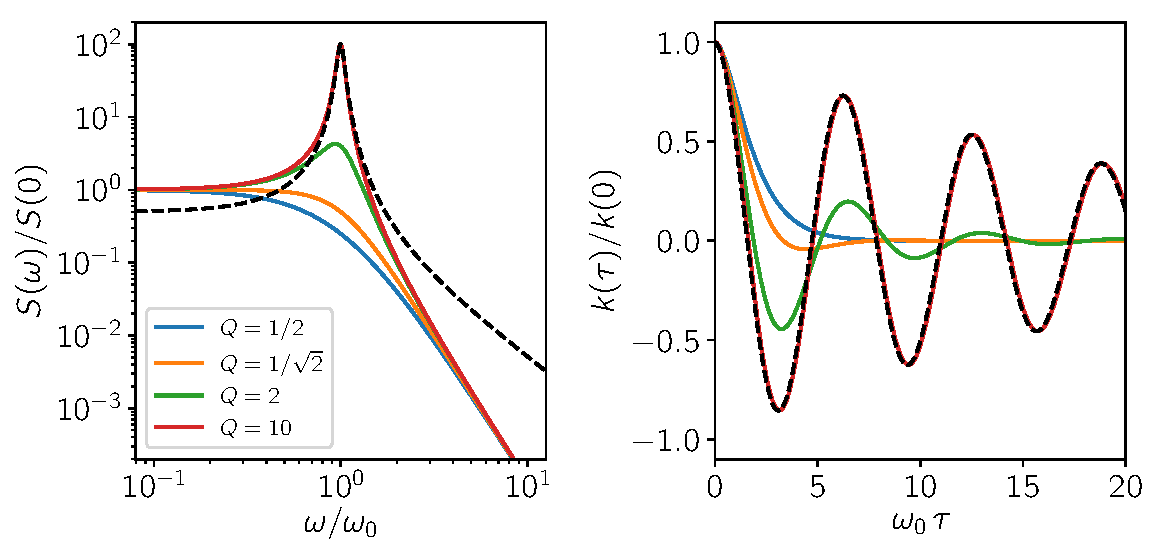
\includegraphics[width=0.95\textwidth]{figures/sho.pdf}
\caption{(left) The power spectrum of a stochastically-driven simple harmonic
    oscillator (\eqalt{sho-psd}) plotted for several values of the quality
    factor $Q$.
    For comparison, the dashed line shows the Lorentzian function from
    \eq{lorentz-psd} with $c_j = \omega_0/(2\,Q) = 1/20$ and normalized so that
    $S(d_j)/S(0) = 100$.
    (middle) The corresponding autocorrelation functions with the same colors.
    \response{(right) Three realizations from each model in the same colors.}
    \figurelabel{sho}}
\end{center}
\end{figure}


\section{Examples}

To demonstrate the application of \celerite, we use it to perform posterior
inference in two examples with realistic simulated data and three examples of
real-world research problems.

start by inferring
posterior constraints on the parameters of a GP model applied to several
simulated datasets with known properties.

In the following section, we expand on these examples by applying
\celerite\ to real datasets.
In the first example, we demonstrate that \celerite\ can be used to infer
the power spectrum of a process when the data are generated from a
\celeriteterm\ model.
In the second example, we demonstrate that \celerite\ can be used as an
effective model even if the true process cannot be represented in the space of
allowed models.
This is an interesting example because, when analyzing real data, we rarely
have any fundamental reason to believe that the data were generated by a GP
model with a specific kernel.
Even in these cases, GPs can be useful effective models and \celerite\
provides computational advantages over other GP methods.

In this section, we demonstrate several use cases of \celerite\ when
applied to real datasets.
Each of these examples touches on an active area of research so we limit our
examples to be qualitative in nature and do not claim that \celerite\ is the
optimum method, but we hope these examples encourage interested readers to
investigate the applicability of \celerite\ to their research.

All of the following examples show time domain datasets with a clear bias in
favor of large homogeneous photometric surveys, but these methods can
similarly be applied to spectroscopy, where wavelength~--~instead of
time~--~is the independent coordinate and other one-dimensional domains
\citep[see][for a potential application]{Czekala:2017}.

\response{In each example, the joint posterior probability density is given by
\begin{eqnarray}\eqlabel{joint-post}
p(\bvec{\theta},\,\bvec{\alpha}\,|\,\bvec{y},\,X) \propto
p(\bvec{y}\,|\,{X,\,\bvec{\theta}},\,\bvec{\alpha})\,
p(\bvec{\theta},\,\bvec{\alpha})
\end{eqnarray}
where $p(\bvec{y}\,|\,{X,\,\bvec{\theta}},\,\bvec{\alpha})$ is the GP
likelihood defined in \eq{gp-likelihood} and
$p(\bvec{\theta},\,\bvec{\alpha})$ is the joint prior probability density for
the parameters.
The specific parameters and priors are discussed in detail in each section
but, in most cases, we assume separable uniform priors with plausibly broad
support.
}

\subsection{Recovery of a celerite process}

In this first example, we simulate a dataset using a known \celeriteterm\
process and fit it with \celerite\ to demonstrate that valid inferences can be
made in this idealized case.
\response{We simulated a small ($N = \exampleindata$) dataset using a GP model
with a SHO kernel (\eqalt{sho-kernel}) with parameters $S_0 =
1\,\mathrm{ppm}^2$, $\omega_0 = e^2\,\mathrm{day}^{-1}$, and $Q = e^2$, where
the units are arbitrarily chosen to simplify the discussion.
We add further white noise with the amplitude $\sigma_n = 2.5\, \mathrm{ppm}$
to each data point.
The simulated data are plotted in the top left panel of
\Figure{simulated-correct}.

In this case, when simulating and fitting, we set the mean function
$\mu_\bvec{\theta}$ to zero~--~this means that the parameter vector
$\bvec{\theta}$ is empty~--~and the elements of the covariance matrix are
given by \eq{sho-kernel} with three parameters $\bvec{\alpha} = (S_0,\,
\omega_0,\,Q)$.
We choose a proper separable prior for $\bvec{\alpha}$ with log-uniform
densities for each parameter as listed in Table~\ref{tab:example-1-params}.

To start, we estimate the maximum \emph{a posteriori} (MAP) parameters using
the \project{L-BFGS-B} non-linear optimization routine \citep{Byrd:1995,
Zhu:1997} implemented by the \project{SciPy} project \citep{Jones:2001}.
The top left panel of \Figure{simulated-correct} shows the conditional mean
and standard deviation of the MAP model over-plotted on the simulated data and
the bottom panel shows the residuals away from this model.
Since we are using the correct model to fit the data, it is reassuring that
the residuals appear qualitatively uncorrelated in this figure.

We then sample the joint posterior probability (\eqalt{joint-post}) using
\emcee\ \citep{Goodman:2010, Foreman-Mackey:2013}.
We initialize \exampleinwalkers~walkers in a Gaussian ball with width
$10^{-4}$ in each parameter around the MAP parameter vector, run
\exampleinburn~steps of burn-in, and \exampleinsteps~steps of MCMC.
To asses convergence, we estimate the mean integrated autocorrelation time of
the chain across parameters \citep{Sokal:1989, Goodman:2010} and find that the
chain results in \exampleineff~effective samples.

Each sample in the chain corresponds to a model PSD and we compare this
posterior constraint on the PSD to the true spectral density in the
right-hand panel of \Figure{simulated-correct}.
In this figure, the true PSD is plotted as a dashed black line and the
numerical estimate of the posterior inference is shown as a blue contour
indicating 68\% of the MCMC samples.
It is clear from this figure that, as expected, the inference correctly
reproduces the true PSD.
}

\begin{floattable}
\begin{deluxetable}{cc}
\tablecaption{The parameters and priors for Example 1. \label{tab:example-1-params}}
\tablehead{\colhead{parameter} & \colhead{prior}}
\startdata
$\ln(S_0)$ & $\mathcal{U}(-10,\,10)$ \\
$\ln(Q)$ & $\mathcal{U}(-10,\,10)$ \\
$\ln(\omega_0)$ & $\mathcal{U}(-10,\,10)$ \\
\enddata
\end{deluxetable}
\end{floattable}


\begin{figure}[!htbp]
\begin{center}
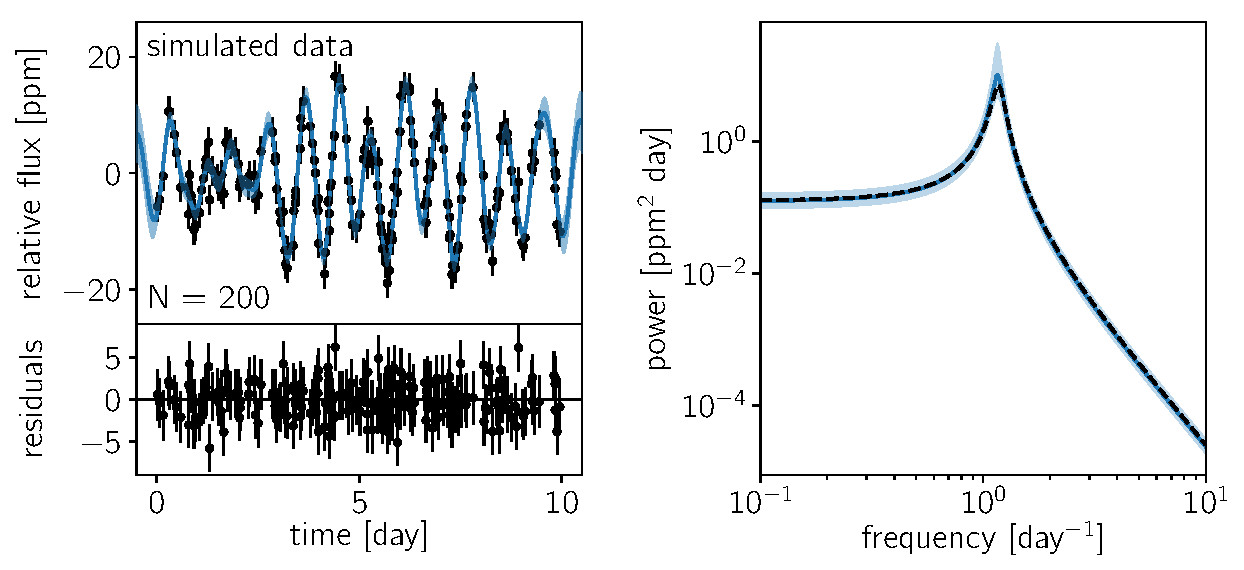
\includegraphics[width=0.9\textwidth]{figures/simulated/correct.pdf}
\caption{(top left) A simulated dataset (black error bars), and maximum
    likelihood model (blue contours).
    (bottom left) The residuals between the mean predictive model and the data
    shown in the top left figure.
    (right) The inferred PSD~--~the blue contours encompass 68\% of the
    posterior mass~--~compared to the true PSD (dashed black line).
    \figurelabel{simulated-correct}}
\end{center}
\end{figure}

\newpage
\subsection{Inferences with the ``wrong'' model}

In this example, we simulate a dataset using a known GP model with a kernel
outside of the support of a \celeriteterm\ process.
This means the true autocorrelation of the process can never be correctly
represented by the model that we are using to fit, but we use this example
to demonstrate that, at least in this case, valid inferences can still be made
about the physical parameters of the model.

The data are simulated from a quasiperiodic GP with the kernel
\begin{eqnarray}\eqlabel{sim-wrong-true}
k_\mathrm{true} (\tau) = \alpha\,
    \exp\left(-\frac{\tau^2}{2\,\lambda^2}\right)\,
    \cos\left(\frac{2\,\pi\,\tau}{P_\mathrm{true}}\right)
\end{eqnarray}
where $P_\mathrm{true}$ is the fundamental period of the process.
This autocorrelation structure corresponds to the power spectrum
\citep{Wilson:2013}
\begin{eqnarray}
S_\mathrm{true} (\omega) = \frac{\lambda\,\alpha}{2}\,\left[
    \exp\left(-\frac{\lambda^2}{2}\,\left(\omega-
        \frac{2\,\pi}{P_\mathrm{true}}\right)^2\right) +
    \exp\left(-\frac{\lambda^2}{2}\,\left(\omega+
        \frac{2\,\pi}{P_\mathrm{true}}\right)^2\right)
\right]
\end{eqnarray}
which, for large values of $\omega$, falls off exponentially. \dfmtodo{$\alpha$
means the parameter vector in definition of likelihood.}
When compared to \eq{celerite-psd}~--~which, for large $\omega$, goes as
$\omega^{-4}$ at most~--~it is clear that a \celeriteterm\ model can never
exactly reproduce the structure of this process.
That being said, we demonstrate that robust inferences can be made about
$P_\mathrm{true}$ even with this effective model.

\response{We generate a realization of a GP model with the kernel given in
\eq{sim-wrong-true} with $N = \exampleiindata$, $\alpha = 1\,\mathrm{ppm}^2$,
$\lambda = 5\,\mathrm{day}$, and $P_\mathrm{true} = 1\,\mathrm{day}$.
We also add white noise with amplitude $\sigma = 0.5\,\mathrm{ppm}$ to each
data point.
The top left panel of \Figure{simulated-wrong} shows this simulated dataset.

We then fit this simulated data using the product of two SHO terms
(\eqalt{sho-kernel}) where one of the terms has $S_0 = 1$ and $Q =
1/\sqrt{2}$ fixed.
The kernel for this model is
\begin{eqnarray}
k(\tau) = k_\mathrm{SHO}(\tau;\,S_0,\,Q,\,\omega_1) \,
    k_\mathrm{SHO}(\tau;\,S_0 = 1,\,Q = 1/\sqrt{2},\,\omega_2)
\end{eqnarray}
where $k_\mathrm{SHO}$ is defined in \eq{sho-kernel} and the inferred period
is related to the parameters by $P=2\,\pi/\omega_1$.
We note that using \eq{product-rule}, the product of two \celeriteterm\ terms
can also be expressed using \celerite.

As in the previous example, we set the mean function to zero and can,
therefore, omit the parameters $\bvec{\theta}$.
Table~\ref{tab:example-2-params} lists the proper log-uniform priors that we
choose for each parameter in $\bvec{\alpha} =
(S_0,\,Q,\,\omega_1,\,\omega_2)$.
These priors, together with the GP likelihood (\eqalt{gp-likelihood}) fully
specify the posterior probability density.

As above, we estimate the MAP parameters using \project{L-BFGS-B} and sample
the posterior probability density using \emcee.
The top left panel of \Figure{simulated-wrong} shows the conditional mean and
standard deviation of the MAP model.
The bottom left panel shows the residuals between the data and this MAP model
and, even though this GP model is formally ``wrong'', there are no obvious
correlations in these residuals.

To perform posterior inference, we initialize \exampleiinwalkers~walkers by
sampling from the 4-dimensional Gaussian centered on the MAP parameters with
an isotropic standard deviation of $10^{-4}$.
We then run \exampleiinburn~steps of burn-in and \exampleiinsteps~steps of
MCMC.
To estimate the number of effective samples, we estimate the integrated
autocorrelation time of the chain for the parameter $\omega_1$~--~the
parameter of primary interest~--~and find \exampleiineff~effective samples.

For comparison, we run the same number of steps of MCMC to sample the
``correct'' joint posterior density.
For this reference inference, we use a GP likelihood with the kernel given by
\eq{sim-wrong-true} and choose log-uniform priors on each of the
three parameters $\ln \alpha/\mathrm{ppm}^2 \sim \mathcal{U}(-10,\,10)$,
$\ln \lambda/\mathrm{day} \sim \mathcal{U}(-10,\,10)$, and
$\ln P_\mathrm{true}/\mathrm{day} \sim \mathcal{U}(-10,\,10)$.

The marginalized posterior inferences of the characteristic period of the
process are shown in the right panel of \Figure{simulated-wrong}.
The inference using the correct model is shown as a dashed blue histogram and
the inference made using the effective model is shown as a solid black
histogram.
These inferences are consistent with each other and with the true period used
for the simulation (shown as a vertical gray line).
This demonstrates that, in this case, \celerite\ can be used as a
computationally efficient effective model and hints that this may be true in
other problems as well.
}

\begin{floattable}
\begin{deluxetable}{cc}
\tablecaption{The parameters for Example 2. \label{tab:example-2-params}}
\tablehead{\colhead{parameter} & \colhead{prior}}
\startdata
$\ln(S_0)$ & $\mathcal{U}(-15,\,5)$ \\
$\ln(Q)$ & $\mathcal{U}(-10,\,10)$ \\
$\ln(\omega_1)$ & $\mathcal{U}(-10,\,10)$ \\
$\ln(\omega_2)$ & $\mathcal{U}(-5,\,5)$ \\
\enddata
\end{deluxetable}
\end{floattable}


\begin{figure}[!htbp]
\begin{center}
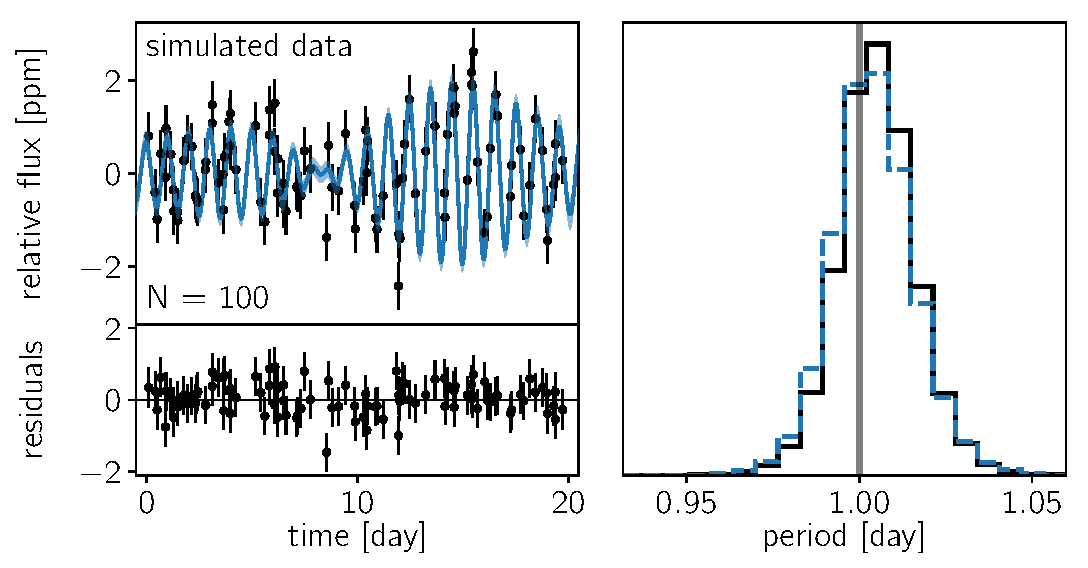
\includegraphics[width=0.9\textwidth]{figures/simulated/wrong-qpo.pdf}
\caption{(top left) A simulated dataset (black error bars), and maximum
    likelihood model (blue contours).
    (bottom left) The residuals between the mean predictive model and the data
    shown in the top left figure.
    (right) The inferred period of the process. The true period is indicated
    by the vertical orange line, the posterior inference using the correct
    model is shown as the blue dashed histogram, and the inference made using
    the ``wrong'' effective model is shown as the black histogram.
    \figurelabel{simulated-wrong}}
\end{center}
\end{figure}


\subsection{Stellar rotation} \sectlabel{rotation}

A source of variability that can be measured from time series measurements of
stars is rotation.
The inhomogeneous surface of the star (spots, plage, \etc) imprints itself as
quasiperiodic variations in photometric or spectroscopic observations
\citep{Dumusque:2014}.
It has been demonstrated that for light curves with nearly uniform sampling,
the empirical autocorrelation function provides a reliable estimate of the
rotation period of a star \citep{Mcquillan:2013, Mcquillan:2014, Aigrain:2015}
and that a GP model with a
quasiperiodic covariance function can be used to make probabilistic
measurements even with sparsely sampled data (R.~Angus, \etal\ submitted).
The covariance function used for this type of analysis has the form
\begin{eqnarray}\eqlabel{sine2}
k(\tau) = A\,\exp\left(-\frac{\tau^2}{2\,\ell^2} -
    \Gamma\,\sin^2\left(\frac{\pi\,\tau}{P} \right) \right)
\end{eqnarray}
where $P$ is the rotation period of the star.
GP modeling with the same kernel function has been proposed as a method of
measuring the mean periodicity in quasiperiodic photometric time series in
general \citep{Wang:2012}.
The key difference between \eq{sine2} and other quasiperiodic kernels is that
it is positive for all values of $\tau$.
We can construct a simple \celeriteterm\ covariance function with similar properties
as follows
\begin{eqnarray}\eqlabel{rot-kernel}
k(\tau) = \frac{a}{2+b}\,e^{-\tau/c}\,\left[
    \cos\left(\frac{2\,\pi\,\tau}{P}\right) + (1 + b)
\right]
\end{eqnarray}
for $a>0$, $b>0$, and $c>0$. \dfmtodo{a,b,c already have different meaning
in celerite kernel.}
The covariance function in \eq{rot-kernel} cannot exactly reproduce \eq{sine2}
but, since \eq{sine2} is only an effective model, \eq{rot-kernel} can be used
as a drop-in replacement for a substantial gain in computational efficiency.

To demonstrate this method, we fit a \celeriteterm\ model with a kernel given
by \eq{rot-kernel} to a \kepler\ light curve for the star KIC~1430163.
This star has a published rotation period of $3.88 \pm 0.58\,\mathrm{days}$,
measured using traditional periodogram and autocorrelation function approaches
applied to \kepler\ data from Quarters 0--16 \citep{Mathur:2014}.
We used \emcee\ to sample the joint posterior probability density for the four
parameters in \eq{rot-kernel}, conditioned on two quarters of \kepler\ data,
and find a constraint on the rotation period of $P = \rotationperiod$.
This is in good agreement with the literature value with somewhat smaller
uncertainties.
A detailed comparison of GP rotation period measurements and the traditional
methods is beyond the scope of this paper, but forthcoming work (R.~Angus,
\etal, submitted) demonstrates that GP inferences are, at a population level,
more reliable than other methods.
The left panels of \Figure{rotation} show a subset of the data used in this
example and the residuals away from the maximum likelihood predictive mean.
The right panel of \Figure{rotation} shows the marginalized posterior
distribution for the rotation period.

\begin{floattable}
\begin{deluxetable}{cc}
\tablecaption{The parameters and priors for Example 3. \label{tab:example-3-params}}
\tablehead{\colhead{parameter} & \colhead{prior}}
\startdata
$\ln(B/\mathrm{ppt}^2)$ & $\mathcal{U}(-10.0,\,0.0)$ \\
$\ln(L/\mathrm{day})$ & $\mathcal{U}(1.5,\,5.0)$ \\
$\ln(P/\mathrm{day})$ & $\mathcal{U}(-3.0,\,5.0)$ \\
$\ln(C)$ & $\mathcal{U}(-5.0,\,5.0)$ \\
\enddata
\end{deluxetable}
\end{floattable}


\begin{figure}[p]
\begin{center}
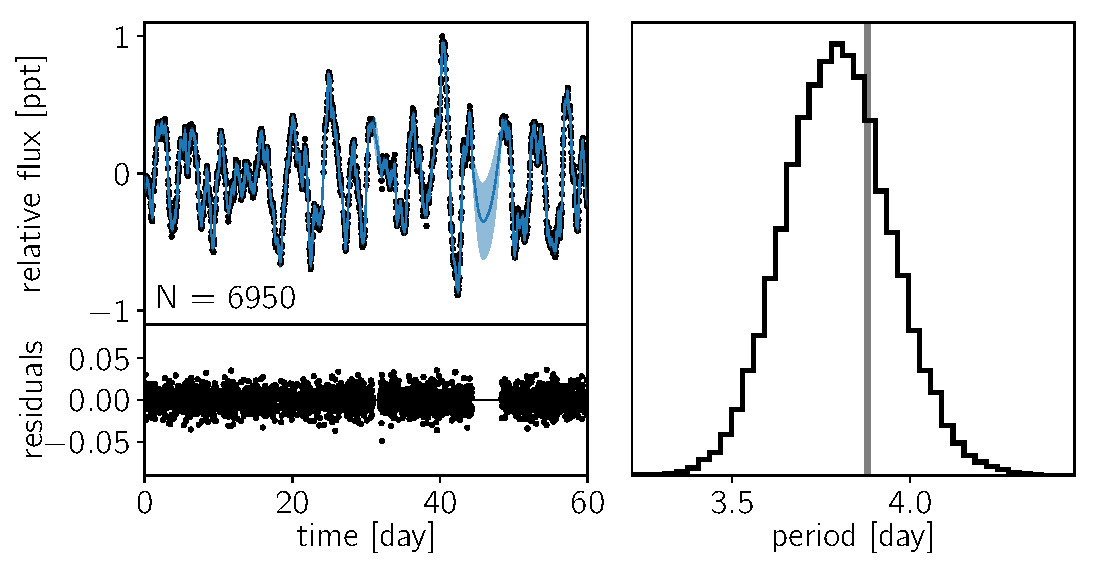
\includegraphics[width=0.8\textwidth]{figures/rotation/rotation.pdf}
\caption{Inferred constraints on a quasiperiodic GP model using the covariance
    function in \eq{rot-kernel} and two quarters of \kepler\ data.
(top left) The \kepler\ data (black points) and the maximum likelihood model
    prediction (blue curve) for a 60~day subset of the data used.
    The solid blue line shows the predictive mean and the blue contours show
    the predictive standard deviation.
(bottom left) The residuals between the mean predictive model and the data
    shown in the top left figure.
(right) The posterior constraint on the rotation period of KIC~1430163 using
    the dataset and model from \Figure{rotation}.
    The period is the parameter $P$ in \eq{rot-kernel} and this figure shows
    the posterior distribution marginalized over all other nuisance parameters
    in \eq{rot-kernel}.
    This is consistent with the published rotation period made using the full
    \kepler\ baseline \citep{Mathur:2014}.
    The error bars from the literature are indicated by the two vertical
    dashed lines.
    \figurelabel{rotation}}
\end{center}
\end{figure}

\subsection{Asteroseismic oscillations}

The asteroseismic oscillations of thousands of stars were measured using light
curves from the \kepler\ mission \citep{Gilliland:2010, Huber:2011,
Chaplin:2011, Chaplin:2013, Stello:2013} and asteroseismology is a key science
driver for many of the upcoming large scale photometric surveys
\citep{Campante:2016, Rauer:2014, Gould:2015}.
Most asteroseismic analyses have been limited to relatively high
signal-to-noise oscillations.
The standard methods use statistics of the empirical periodogram and cannot
formally propagate the measurement uncertainties to the constraints on
physical parameters, instead relying on bootstrapped uncertainty estimators
\citep{Huber:2009}.
More sophisticated methods that compute the likelihood function in the time
domain scale poorly to state-of-the-art datasets \citep{Brewer:2009,
Corsaro:2014}.

\celerite\ alleviates these problems by providing a physically motivated
probabilistic model that can be evaluated efficiently even for large datasets.
In practice, one would model the star as a mixture of stochastically-driven
simple harmonic oscillators where the amplitudes and frequencies of the
oscillations are computed using a physical model, and evaluate the probability
of the observed time series using a GP where the PSD is a sum of terms given
by \eq{sho-psd}.
This gives us a method of computing the likelihood function for the parameters
of the physical model (for example, $\nu_\mathrm{max}$ and $\Delta \nu$, or
other more fundamental parameters) \emph{conditioned on the observed time
series} in $\mathcal{O}(N)$ operations.
In other words, \celerite\ provides a computationally efficient framework that
can be combined with physically-motivated models of stars and numerical
inference methods to make rigorous probabilistic measurements of asteroseismic
parameters in the time domain.
We expect that this has the potential to push asteroseismic analysis to lower
signal-to-noise datasets and we hope to revisit this idea in a subsequent
paper.

To demonstrate the method, we use a simple heuristic model where the PSD is
given by a mixture of 8 components with amplitudes and frequencies specified
by $\nu_\mathrm{max}$, $\Delta \nu$, and several nuisance parameters.
The first term is used to capture the granulation ``background''
\citep{Kallinger:2014} using \eq{granulation-psd} with two free parameters
$S_g$ and $\omega_g$.
The remaining  7 terms are given by \eq{sho-psd} where $Q$ is a nuisance
parameter shared between terms and the frequencies are given by
\begin{eqnarray}
\omega_{0,\,j} = 2\,\pi\,(\nu_\mathrm{max} + j\,\Delta\nu + \epsilon)
\end{eqnarray}
and the amplitudes are given by
\begin{eqnarray}
S_{0,\,j} =
    \frac{A}{Q^2}\,\exp\left(-\frac{[j\,\Delta\nu + \epsilon]^2}{2\,W^2}\right)
\end{eqnarray}
where $j$ is an integer running from $-3$ to 3 and $\epsilon$, $A$, and $W$
are shared nuisance parameters. \dfmtodo{A was used for diagonal of
covariance matrix.}
This model could be extended to include more angular modes and
$\nu_\mathrm{max}$ and $\Delta \nu$ could be replaced by the fundamental
physical parameters of the star.

To demonstrate the applicability of this model, we apply it to infer the
asteroseismic parameters of the giant star KIC~11615890, observed by the
\kepler\ Mission.
The goal of this example is to show that, even for a low signal-to-noise
dataset with a short baseline, it is possible to infer asteroseismic
parameters with formal uncertainties that are consistent with the parameters
inferred with a much larger dataset.
Looking forward to \tess\ \citep{Ricker:2014,Campante:2016}, we measure
$\nu_\mathrm{max}$ and $\Delta\nu$ using only one month of \kepler\ data and
compare our results to the results inferred from the full 4 year baseline of
the \kepler\ mission.
Unlike typical giants, KIC~11615890 is a member of a class of stars where the
dipole ($\ell = 1$) oscillation modes are suppressed by strong magnetic fields
in the core \citep{Stello:2016}.
This makes this target simpler for the purposes of this demonstration because
we can neglect the $\ell = 1$ modes and the model proposed above will be an
effective model for the combined signal from the $\ell = 0$ and 2 modes.

For KIC~11615890, the published asteroseismic parameters measured using several
years of \kepler\ observations are \citep{Pinsonneault:2014}
\begin{eqnarray}
    \nu_\mathrm{max} = 171.94 \pm 3.62 \,\mu\mathrm{Hz} \quad\mathrm{and}\quad
    \Delta\nu = 13.28 \pm 0.29 \,\mu\mathrm{Hz} \quad.
\end{eqnarray}
We randomly select a month-long segment of PDC \citep{Stumpe:2012, Smith:2012}
\kepler\ data, initialize our \celeriteterm\ model using a grid search in the
parameter space, and then use \emcee\ \citep{Foreman-Mackey:2013} to sample
the joint posterior density for the full set of parameters.
\Figure{astero-corner} shows the marginalized density for $\nu_\mathrm{max}$
and $\Delta\nu$ compared to the results from the literature.
This result is consistent within the published error bars and the posterior
constraints are tighter than the published results.
All asteroseismic analyses are known to have substantial systematic and
method-dependent uncertainties \citep{Verner:2011} so further experiments
would be needed to assess the reliability of this method.

This model requires about a minute of computation time to find the maximum
likelihood parameters and then it takes about an hour to run the MCMC sampling
to convergence on a dual-CPU laptop.
This is more computationally intensive than traditional methods of measuring
asteroseismic oscillations, but is is also orders of magnitude cheaper than the
same analysis using another GP solver.
An in-depth discussion of the benefits of rigorous probabilistic inference of
asteroseismic parameters in the time domain is beyond the scope of this paper,
but we hope to revisit this opportunity in the future.

\begin{floattable}
\begin{deluxetable}{cc}
\tablecaption{The parameters for Example 4. \label{tab:example-4-params}}
\tablehead{\colhead{parameter} & \colhead{prior}}
\startdata
$\ln(S_g/\mathrm{ppm}^2)$ & $\mathcal{U}(-15,\,15)$ \\
$\ln(\omega_g/\mathrm{day}^{-1})$ & $\mathcal{U}(-15,\,15)$ \\
$\ln(\nu_\mathrm{max}/\mu\mathrm{Hz})$ & $\mathcal{U}(\ln(130),\,\ln(190))$ \\
$\ln(\Delta \nu/\mu\mathrm{Hz})$ & $\mathcal{U}(\ln(12.5),\,\ln(13.5))$ \\
$\epsilon/\mathrm{day}^{-1}$ & $\mathcal{N}(0,\,1)$ \\
$\ln(A/\mathrm{ppm}^2\,\mathrm{day})$ & $\mathcal{U}(-15,\,15)$ \\
$\ln(Q)$ & $\mathcal{U}(-15,\,15)$ \\
$\ln(W/\mathrm{day}^{-1})$ & $\mathcal{U}(-3,\,3)$ \\
$\ln(\sigma/\mathrm{ppm})$ & $\mathcal{U}(-15,\,15)$ \\
\enddata
\end{deluxetable}
\end{floattable}


\begin{figure}[!htbp]
\begin{center}
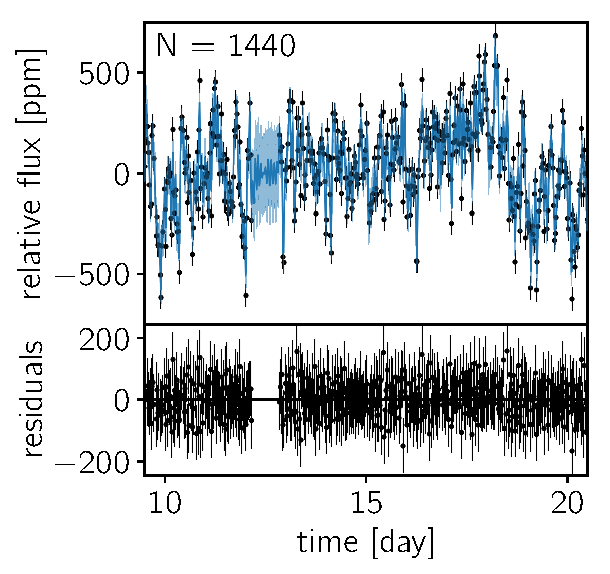
\includegraphics[width=0.8\textwidth]{figures/astero/astero.pdf}
\caption{
\response{
(top) The \kepler\ data (black points) and the maximum likelihood model
    prediction (blue curve) for a 10~day subset of the month-long dataset that
    was used for the fit.
    The solid blue line shows the predictive mean and the blue contours show
    the predictive standard deviation.
(bottom) The residuals between the mean predictive model and the data
    shown in the top figure.
}
    \figurelabel{astero}}
\end{center}
\end{figure}

\begin{figure}[!htbp]
\begin{center}
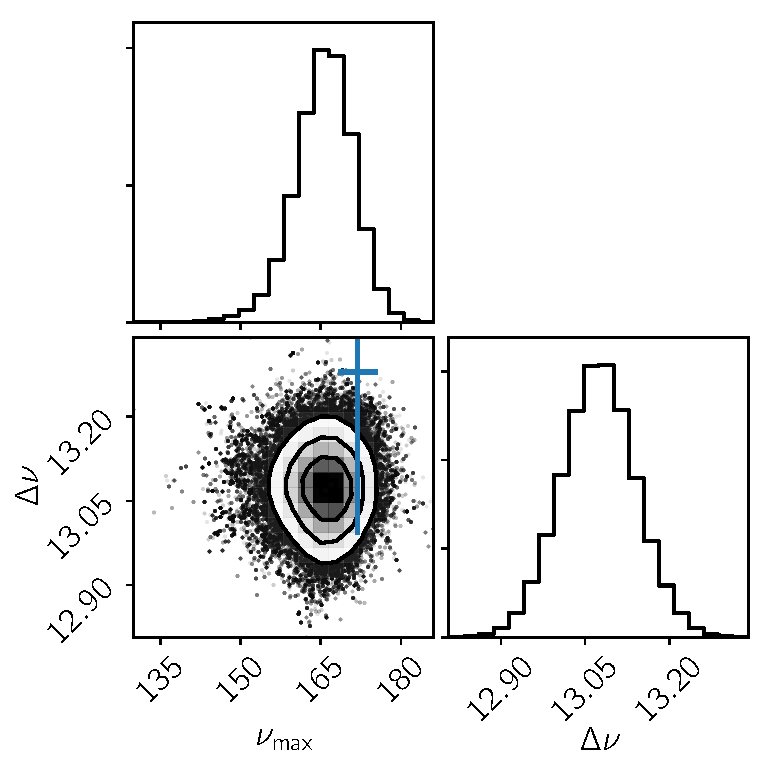
\includegraphics[width=0.8\textwidth]{figures/astero/astero-corner.pdf}
\caption{The probabilistic constraints on $\nu_\mathrm{max}$ and $\Delta \nu$
    from the inference shown in \Figure{astero} compared to the published
    value (error bar) based on several years of \kepler\ observations
    \citep{Pinsonneault:2014}.
    \figurelabel{astero-corner}}
\end{center}
\end{figure}

\begin{figure}[!htbp]
\begin{center}
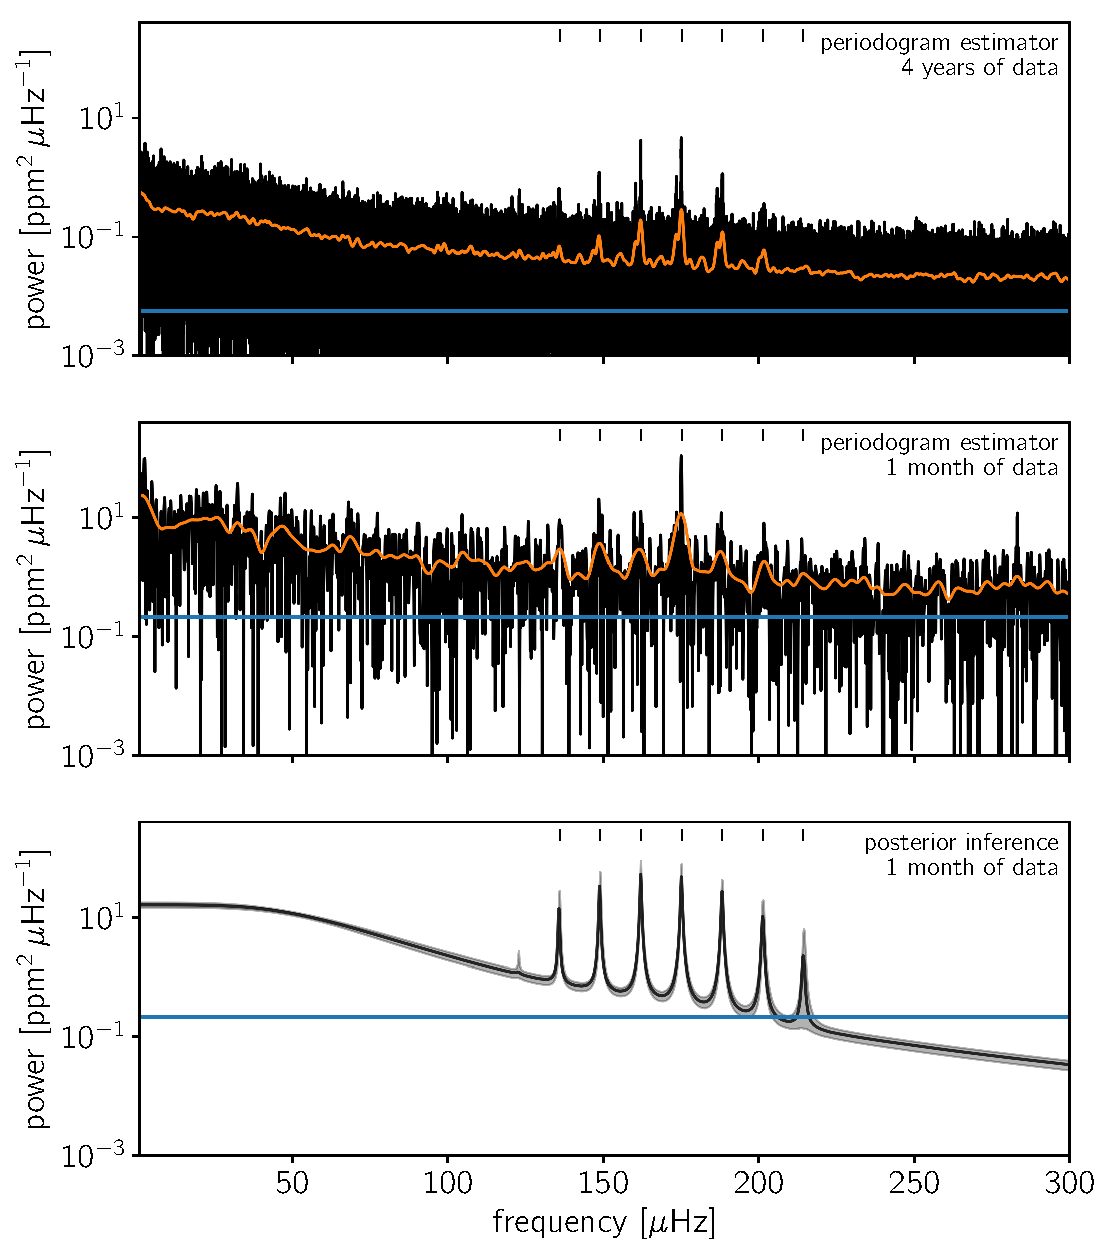
\includegraphics[width=0.9\textwidth]{figures/astero/astero-comp.pdf}
\caption{A comparison between the Lomb-Scargle estimator of the PSD and the
posterior inference of the PSD as a mixture of stochastically-driven simple
harmonic oscillators.
(top) The periodogram of the \kepler\ light curve for KIC~11615890 computed
    on the full four year baseline of the mission. The orange line shows a
    smoothed periodogram and the blue line indicates the level of the
    measurement uncertainties.
(middle) The same periodogram computed using about a month of data.
(bottom) The power spectrum inferred using the mixture of SHOs model described
    in the text and only one month of \kepler\ data.
    The black line shows the median of posterior PSD and the gray contours
    show the 68\% credible region.
    \figurelabel{astero}}
\end{center}
\end{figure}


\subsection{Exoplanet transit fitting}

In this example, we inject the signal of a simulated exoplanet transit into a
real \kepler\ light curve and then demonstrate that we can recover the true
physical parameters of the exoplanet while modeling the stellar variability
using \celerite.
This example is different from all the previous examples~--~both simulated and
real~--~because, in this case, we are uninterested in the parameters of the
covariance model.
Instead, we're interested in inferring constraints on the parameters of the
mean model ($\mu_\bvec{\theta}(\bvec{x})$ from \sect{gps}), the model of the
signal caused by the transit of the planet.
We say ``mean model'' here to unambiguously distinguish it from the
``covariance model'', but this is what would generally be called the ``model''
in other analyses.
In this case, we have a light curve of a rotating star with a planet
transiting and we would like to fit for the physical parameters of the planet
while taking our uncertainty about the star's variability into account.
GP modeling has been used for this purpose throughout the exoplanet literature
\citep[for example][]{Dawson:2014, Barclay:2015, Evans:2015,
Foreman-Mackey:2016b, Grunblatt:2016}.

In \eq{gp-likelihood} the physical parameters of the planet are called
$\bvec{\theta}$ and, in this example, the mean function $\mu_\bvec{\theta}(t)$
is a limb-darkened transit light curve \citep{Mandel:2002} and the parameters
$\bvec{\theta}$ are a period $P$, a transit duration $T$, a phase or epoch
$t_0$, an impact parameter $b$, the radius of the planet in units of the
stellar radius $R_P/R_\star$, and several parameters describing the
limb-darkening profile of the star \citep{Claret:2011}.
As in the previous example, we model the stellar variability using a GP model
with a kernel given by \eq{rot-kernel} and fit for the parameters of the
planet $\bvec{\theta}$ and the stellar variability $\bvec{\alpha}$
simultaneously.

We take a month-long segment of the \kepler\ light curve for
KIC~1430163~--~the target from \sect{rotation}~--~and multiply it by a
simulated transit model with known parameters.
The fact that we are using a simulated transit enables us to confirm that we
correctly measure the planet parameters but we do not use this knowledge to
inform our fit.
The top panel of \Figure{transit-ml} shows the data including the simulated
transit.
The bottom panel shows the same data with the maximum likelihood prediction
for the stellar variation subtracted.
To find this model, we maximized the likelihood function in \eq{gp-likelihood}
with respect to the transit parameters $\bvec{\theta}$ and the variability
parameters $\bvec{\alpha}$ simultaneously.
\Figure{transit-corner} shows the marginalized posterior constraints on the
physical properties of the planet compared to the true values.
This procedure produces estimates of the planet parameters that are consistent
with the true values using \celerite\ as an effective model for the stellar
variability.

\newpage

\dfmtodo{Table 5 has two parameter with name "b":  the celerite coefficient,
and the impact parameter.}

\begin{floattable}
\begin{deluxetable}{cc}
\tablecaption{The parameters and priors for Example 5. \label{tab:example-5-params}}
\tablehead{\colhead{parameter} & \colhead{prior}}
\startdata
$\ln(a/\mathrm{ppt}^2)$ & $\mathcal{U}(-10.0,\,0.0)$ \\
$\ln(c/\mathrm{day})$ & $\mathcal{U}(1.5,\,5.0)$ \\
$\ln(P_\mathrm{rot}/\mathrm{day})$ & $\mathcal{U}(-3.0,\,5.0)$ \\
$\ln(b)$ & $\mathcal{U}(-5.0,\,5.0)$ \\
$\ln(\sigma/\mathrm{ppt})$ & $\mathcal{U}(-5.0,\,0.0)$ \\
$f_0/\mathrm{ppt}$ & $\mathcal{U}(-0.5,\,0.5)$ \\
$\ln(P_\mathrm{orb}/\mathrm{day})$ & $\mathcal{U}(\ln(7.9),\,\ln(8.1))$ \\
$\ln(R_p/R_\star)$ & $\mathcal{U}(\ln(0.005),\,\ln(0.1))$ \\
$\ln(T/\mathrm{day})$ & $\mathcal{U}(\ln(0.4),\,\ln(0.6))$ \\
$t_0/\mathrm{day}$ & $\mathcal{U}(-0.1,\,0.1)$ \\
$B$ & $\mathcal{U}(0,\,1.0)$ \\
$q_1$ & $\mathcal{U}(0,\,1)$ \\
$q_2$ & $\mathcal{U}(0,\,1)$ \\
\enddata
\end{deluxetable}
\end{floattable}


\begin{figure}[!htbp]
\begin{center}
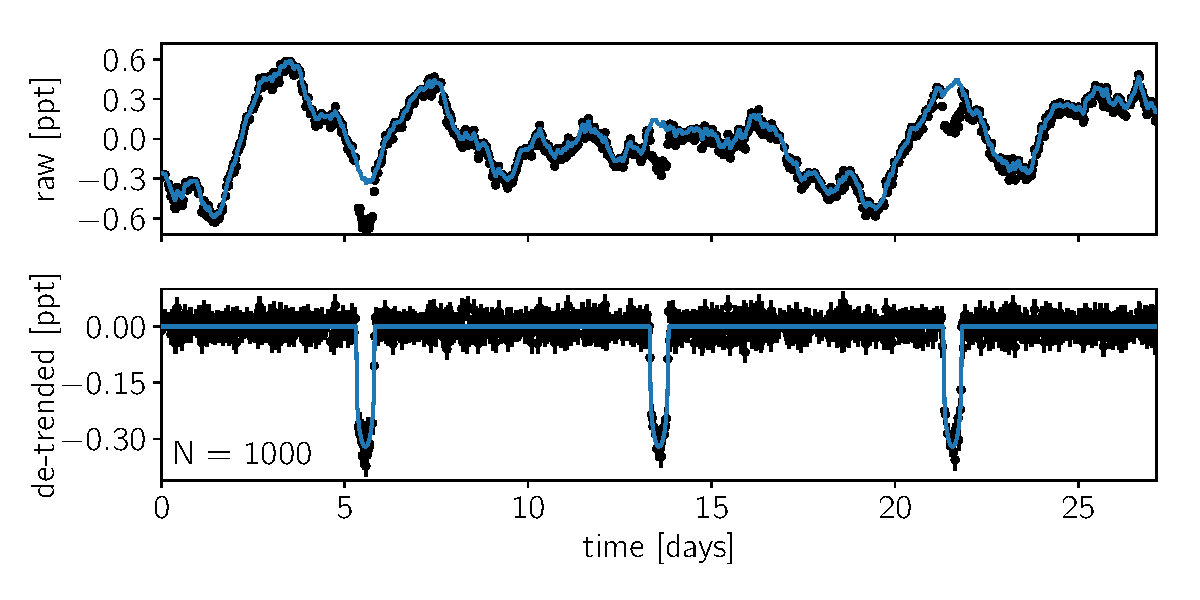
\includegraphics[width=\textwidth]{figures/transit/transit-ml.pdf}
    \caption{\emph{(top)} A month-long segment of \kepler\ light curve for
    KIC~1430163 with a synthetic transit model injected (black points) and the
    maximum likelihood model for the stellar variability
    (blue line).
    \emph{(bottom)} The maximum likelihood ``de-trending'' of the data in
    the top panel.
    In this panel, the maximum likelihood model for the stellar variability
    has been subtracted to leave only the transits.
    The de-trended light curve is shown by black error bars and the maximum
    likelihood transit model is shown as a blue line.
    \figurelabel{transit-ml}}
\end{center}
\end{figure}

\begin{figure}[!p]
\begin{center}
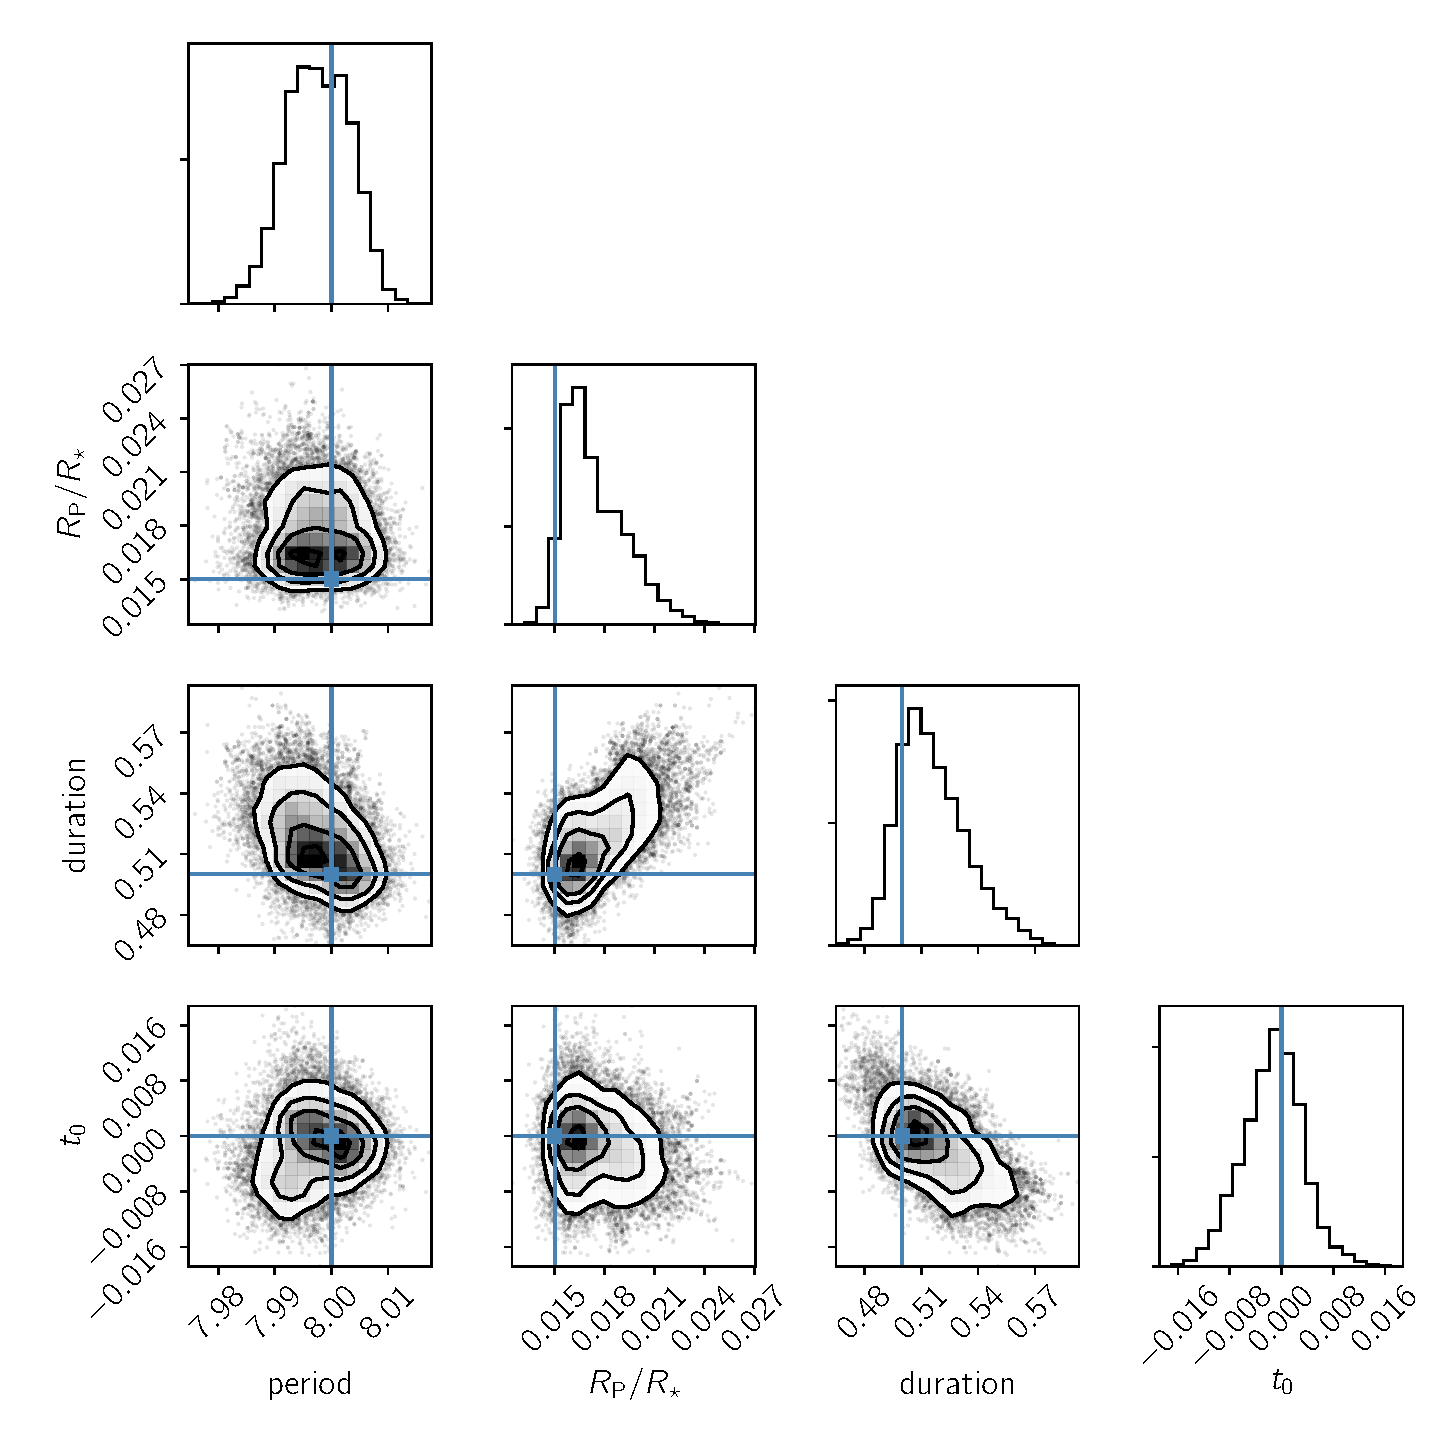
\includegraphics[width=\textwidth]{figures/transit/transit-corner.pdf}
\caption{The marginalized posterior constraints on the physical parameters of
    the planet transit in the light curve shown in the top panel of
    \Figure{transit-ml}.
    The two-dimensional contours show the 0.5-, 1-, 1.5, and 2-sigma credible
    regions in the marginalized planes and the histograms along the diagonal
    show the marginalized posterior for each parameter.
    The true values used in the simulation are indicated by blue lines.
    For each parameter, the inference is consistent with the true value.
    \figurelabel{transit-corner}}
\end{center}
\end{figure}

\subsection{Summary}

\dfmtodo{The D in Table 6 may be confused with the D used in the Cholesky solver.}

\begin{floattable}
\begin{deluxetable}{cccccccc}
\caption{The scaling and convergence stats for each example. \label{tab:example-stats}}
\tablehead{\colhead{example} & \colhead{$N$} & \colhead{$J$} & \colhead{direct cost} & \colhead{\celerite\ cost} & \colhead{$D$} & \colhead{steps} & \colhead{effective samples}\\
&&& \colhead{ms} & \colhead{ms} &&&}
\startdata
1 & 200 & 1 & 2.85 & 0.26 & 3 & 80000 & 1737 \\
2 & 100 & 2 & 0.67 & 0.36 & 4 & 80000 & 1134 \\
3 & 6950 & 2 & 7351.71 & 1.46 & 4 & 176000 & 3606 \\
4 & 1440 & 8 & 828.93 & 2.74 & 9 & 640000 & 1443 \\
5 & 1000 & 2 & 82.73 & 0.94 & 13 & 640000 & 1141 \\
\enddata
\end{deluxetable}
\end{floattable}


\section{Comparisons to other methods}

There are many other methods of scaling GP models to large datasets and in
this section we draw comparisons between \celerite\ and other popular methods.
Scalable GP methods tend to fall into two categories: approximate and
restrictive.
\celerite\ falls into the latter category because, while the method is exact,
it requires a specific choice of stationary kernel function and it can only be
used in one-dimension.

As discussed previously, the \celerite\ method is based upon a method
developed by Rybicki \& Press twenty years ago \citep{Rybicki:1995}.
In the case where the kernel function has a single term of the form given in
\eq{kernel-simple}, it is interesting to compare the performance of \celerite\
and the Rybicki \& Press method.
Their method does not require solving the extended matrix because the matrix
inverse can be calculated analytically, but the method is made slightly more
complicated when white noise is included.
We implement their full method and find empirically that it is more
computationally efficient by a factor of $\approx 2$ for large $N \gg 1000$,
but we note that the requirement of a single, real, exponential kernel is
extremely restrictive and this model cannot describe quasi-periodic
variability.

Another popular method uses the fact that, in the limit of evenly-spaced data
and homoscedastic uncertainties, the covariance matrix is ``Toeplitz''
\citep[for example][]{Dillon:2013}.
There are exact methods for solving Toeplitz matrix equations that scale as
$\mathcal{O}(N\,\log N)$ and methods for computing determinants exactly in
$\mathcal{O}(N^2)$ or approximately in $\mathcal{O}(N\,\log N)$
\citep{Wilson:2014}.
The Toeplitz method is, in some ways, more flexible than \celerite\ because it
can be used with any stationary kernel, but it requires uniformly spaced data
and the scaling is worse than \celerite\ so it is less efficient when applied
to large datasets.

\citet{Carter:2009} improved the scaling of Toeplitz methods by introducing a
wavelet-based method for computing a GP likelihood with $\mathcal{O}(N)$
scaling.
This method has been widely applied in the context of exoplanet transit
characterization, but it requires evenly spaced observations and the power
spectrum of the process must have the form $S(\omega)\propto \omega^{-1}$ to
gain the computational advantage.
This wavelet method has been demonstrated to improve parameter estimation for
transiting exoplanets \citep{Carter:2009}, but these strict requirements make
this method applicable for only a limited set of use cases.

The continuous autoregressive moving average (CARMA) models introduced into
the astrophysics literature by \citet{Kelly:2014} share many features with
\celerite.
CARMA models are derived by solving a stochastic differential equation and,
like \celerite, the likelihood function for a CARMA model conditioned on a
one-dimensional dataset can be solved in $\mathcal{O}(N)$.
The kernel function for a CARMA$(J,\,K)$ model is \citep{Kelly:2014}
\begin{eqnarray}\eqlabel{carma-kernel}
k_\mathrm{CARMA}(\tau) = \sum_{j=1}^J A_j\,\exp\,(r_j\,\tau)
\end{eqnarray}
where
\begin{eqnarray}\eqlabel{carma-coeff}
A_j = \sigma^2 \,\frac{\left[\sum_{k=0}^K\beta_k\,{(r_j)}^k\right]\,
    \left[\sum_{k=0}^K\beta_k\,{(-r_j)}^k\right]}
    {-2\,\mathrm{Re}(r_j)\,\prod_{k=1,\,k \ne j}^{J}(r_k-r_j)({r_k}^*+r_j)}
\end{eqnarray}
and $\sigma$, $\{r_j\}_{j=1}^J$ and $\{\beta_k\}_{k=1}^K$ are parameters of
the model.
Comparing \eq{carma-kernel} to \eq{celerite-kernel-complex}, we can see that
every CARMA model corresponds to an equivalent \celeriteterm\ model and the
parameters $a_j$, $b_j$, $c_j$, and $d_j$ can be easily computed analytically.
The inverse statement is not as simple.
In practice, this means that \celerite\ could be trivially used to compute any
CARMA model.
Using the CARMA solver to compute a \celeriteterm\ model, however, requires
solving \eq{carma-coeff} numerically for a given set of $\{A_j\}_{j=1}^J$.
While the computational scaling of CARMA models is also $\mathcal{O}(N\,J^2)$,
the Kalman filtering based method for solving CARMA models \citep{Kelly:2014}
is, in practice, somewhat faster and the memory requirements are smaller.
One benefit of the \celeriteterm\ model is that it is parameterized in terms
of the amplitudes directly.
This means that the physical interpretation of these parameters is, in some
cases, simpler.
On the other hand, CARMA models are parameterized by modeling the power
spectrum of the stochastic driving force and this might be the quantity of
interest in other situations.
Another benefit of the \celeriteterm\ framework is that, unlike
filtering-based CARMA solvers, it directly solves matrix equations of the form
${K_\bvec{\alpha}}^{-1}\,b$ in $\mathcal{O}(N)$.
This is a crucial feature when GP modeling is combined with linear models
\citep[for example][]{Luger:2017}.

Another GP method that has been used extensively in astronomy is the
hierarchical off-diagonal low rank \citep[HODLR,][]{Ambikasaran:2016} solver.
This method exploits the fact that many commonly used kernel functions produce
``smooth'' matrices to approximately compute the GP likelihood with the
scaling $\mathcal{O}(N\,\log^2 N)$.
This method has the advantage that, unlike \celerite, it can be used with any
kernel function but, in practice, the cost can still prove to be prohibitively
high for multi-dimensional inputs.
The proportionality constant in the $N\,\log^2N$ scaling of the HODLR method
is a function of the specific kernel and we find~--~using the \project{george}
software package \citep{Foreman-Mackey:2014, Ambikasaran:2016}~--~that this
scales approximately linearly with $J$, but it requires substantial overhead
for small models.
This means that the HODLR solver can \emph{approximately} evaluate
\celeriteterm\
models more efficiently than \celerite\ for large models $J \gg 10$ and
small datasets where $N$ is smaller than a few thousand.

The structured kernel interpolation \citep[SKI/KISS-GP][]{Wilson:2015}
framework is another approximate method that can be used to scale GPs to large
datasets.
This method uses fast interpolation of the kernel into a space where Toeplitz
or Kronecker structure can be used to scale inference and prediction.
The SKI/KISS-GP framework can be applied to scale GP inference with a wide
range of kernels, but the computational cost will depend on the specific
dataset, model, and precision requirements for the approximation.
The SKI method has an impressive $\mathcal{O}(1)$ cost for test-time
predictions and it is interesting to consider how this could be applied to
\celeriteterm\ models.

Many other approximate methods for scaling GP inference exist \citep[see, for
example,][and references therein]{Wilson:2015a} and we make no attempt to make
our discussion exhaustive.
The key takeaway here is that \celerite\ provides an \emph{exact} method for
GP inference for a specific, but flexible, class of one-dimensional kernel
functions.
Furthermore, since \celeriteterm\ models can be interpreted as a mixture of
stochastically-driven, damped simple harmonic oscillators, they are a
physically motivated choice of covariance function in many applications.

\section{Summary}

Gaussian Process models have been fruitfully applied to many problems in
astronomical data analysis, but the fact that the computational cost scales as
the cube of the number of data points has limited their use to relatively
small datasets.
With the linear scaling of \celerite\, we envision the application of Gaussian
processes may be expanded to much larger datasets.
Despite the restrictive form of the \celeriteterm\ kernel, with a sufficient
number of components it is flexible enough to describe a wide range of
astrophysical variability.
In fact, the relation of the \celeriteterm\ kernel to the damped, stochastically-driven harmonic
oscillator matches simple models of astrophysical variability, and makes the
parameterization interpretable in terms of resonant frequency, amplitude, and
quality factor.
% Siva: Removed major, since $J$ is most often small as stated in the second half of the sentence
A drawback of this method is its quadratic scaling with the number of
terms $J$, but, in many cases, small values of $J$ are sufficient.

Our background is in studying transiting exoplanets, a field which has only
recently begun to adopt full covariance matrices in analyzing the noise in
stellar light curves when detecting or characterizing transiting planets
\citep[for example,][]{Carter:2009, Gibson:2012, Barclay:2015, Evans:2015,
Aigrain:2016, Foreman-Mackey:2016b, Grunblatt:2016, Luger:2016}.
All of these analyses have been limited to small datasets or restrictive
kernel choices.
\celerite\ weakens these requirements by providing a scalable method for
computing the likelihood and a physical motivation for the choice of kernel.
\celerite\ can be used to model stellar oscillations using the relation to the
mixture of stochastically-driven, damped simple harmonic oscillators.
As higher signal-to-noise observations of transiting exoplanet systems are
obtained, the effects of stellar variability will more dramatically impact the
correct inference of planetary transit parameters.
We expect that \celerite\ will be important for transit detection
\citep{Pope:2016, Foreman-Mackey:2016b}, transit timing \citep{Agol:2005,
Holman:2005}, transit spectroscopy \citep{Brown:2001}, Doppler beaming
\citep{Loeb:2003, Zucker:2007}, tidal distortion \citep{Zucker:2007}, phase
functions \citep{Knutson:2007, Zucker:2007}, and more.

Beyond these applications to model stellar variability, the method is
generally applicable to other one-dimensional GP models.
Accreting black holes show time series which may be modeled using a GP
\citep{Kelly:2014}; indeed, this was the motivation for the original technique
developed by Rybicki \& Press \citep{Rybicki:1992, Rybicki:1995}.
This approach may be broadly used for characterizing quasar variability
\citep{MacLeod:2010}, measuring time lags with reverberation mapping
\citep{Zu:2011, Pancoast:2014}, modeling time delays in multiply-imaged
gravitationally-lensed systems \citep{Press:1998}, characterizing
quasi-periodic variability in a high-energy source \citep{McAllister:2016}, or
classification of variable objects \citep{Zinn:2016}.
We expect that there are also applications beyond astronomy.

The \celeriteterm\ formalism can also be used for power spectrum estimation and
quantification of its uncertainties.
In principle, a large number of \celeriteterm\ terms could be used to perform
non-parametric probabilistic inference of the power spectrum despite
unevenly-spaced data with heteroscedastic noise \citep[for
example,][]{Wilson:2013, Kelly:2014}.
This type of analysis will be limited by the quadratic scaling of \celerite\
with the number of terms $J$, but this limits existing methods as well
\citep[CARMA models,][]{Kelly:2014}.
In general, we encourage the use of physically motivated models for parameter
estimation instead of qualitative modeling of the power spectrum itself.

There are many data analysis problems where \celerite\ will not be applicable.
In particular, the restriction to one-dimensional problems is significant.
There are many examples of multidimensional GP modeling the astrophysics
literature \citep[recent examples from the field of exoplanet characterization
include][]{Haywood:2014, Rajpaul:2015, Aigrain:2016}, where \celerite\ cannot
be used to accelerate any of these analyses.
It is plausible that an extension could be derived to tackle some
multidimensional problems with the right structure~--~simultaneous parallel
time series, for example~--~and we hope to revisit this possibility in future
work.

Alongside this paper, we have released a well-tested and documented open
source software package that implements the method and all of the examples
discussed in these pages.
This software is available on GitHub
\url{https://github.com/dfm/celerite}\footnote{This version of the paper was
generated with git commit \texttt{\githash} (\gitdate).} and Zenodo
\citep{Foreman-Mackey:2017}, and it is made available under the MIT license.

\acknowledgments
It is a pleasure to thank
Megan Bedell,
Ian Czekala,
Will Farr,
Sam Grunblatt,
David W.\ Hogg,
Dan Huber,
Meredith Rawls,
Dennis Stello,
Jake VanderPlas, and
Andrew Gordon Wilson
for helpful discussions informing the ideas and code presented here.
\response{We would also like to thank the anonymous referee for thorough and
constructive feedback that greatly improved the paper.}

This work was performed in part under contract with the Jet Propulsion
Laboratory (JPL) funded by NASA through the Sagan Fellowship Program executed
by the NASA Exoplanet Science Institute.
EA acknowledges support from NASA grants NNX13AF20G, NNX13A124G, NNX13AF62G,
from National Science Foundation (NSF) grant AST-1615315, and from
NASA Astrobiology Institute's Virtual Planetary Laboratory, supported
by NASA under cooperative agreement NNH05ZDA001C.

This research made use of the NASA \project{Astrophysics Data System} and the
NASA Exoplanet Archive.
The Exoplanet Archive is operated by the California Institute of Technology,
under contract with NASA under the Exoplanet Exploration Program.

This paper includes data collected by the \kepler\ mission. Funding for the
\kepler\ mission is provided by the NASA Science Mission directorate.
We are grateful to the entire \kepler\ team, past and present.
These data were obtained from the Mikulski Archive for Space Telescopes
(MAST).
STScI is operated by the Association of Universities for Research in
Astronomy, Inc., under NASA contract NAS5-26555.
Support for MAST is provided by the NASA Office of Space Science via grant
NNX13AC07G and by other grants and contracts.

This research made use of Astropy, a community-developed core Python package
for Astronomy \citep{Astropy-Collaboration:2013}.

\facility{Kepler}
\software{%
     \project{AstroPy} \citep{Astropy-Collaboration:2013},
     \project{corner.py} \citep{Foreman-Mackey:2016},
     \project{Eigen} \citep{Guennebaud:2010},
     \project{emcee} \citep{Foreman-Mackey:2013},
     \project{george} \citep{Ambikasaran:2016},
     \project{LAPACK} \citep{Anderson:1999},
     \project{matplotlib} \citep{Hunter:2007},
     \project{numpy} \citep{Van-Der-Walt:2011},
     \project{transit} \citep{Foreman-Mackey:2016a},
     \project{scipy} \citep{Jones:2001}.
}

\newpage
\appendix

\section{An alternative solver using the extended matrix formalism}

\citet{Rybicki:1995} demonstrated that the inverse of a matrix $K$, with
elements given by \eq{kernel-simple}, could be computed
efficiently by taking advantage of the structure of this covariance function.
\citet{Ambikasaran:2015} generalized this computation to apply to the full
mixture of $J$ terms in \eq{celerite-kernel-complex} and derived an equally
efficient method for computing the determinant of $K$.

\subsection{An example}

To provide some insight for this method, we follow
\citet{Ambikasaran:2015} and start by working through a simple example.
In this case, we assume that we have three data points
$\{y_1,\,y_2,\,y_3\}$ observed at times $\{t_1,\,t_2,\,t_3\}$ with measurement
variances $\{{\sigma_1}^2,\,{\sigma_2}^2,\,{\sigma_3}^2\}$ and we would
like to compute the likelihood of these data under a GP model with the
covariance function
\begin{eqnarray}
k(\tau_{nm}) = \sigma_n^2\,\delta_{nm} + a\,\exp(-c\,\tau_{nm})\quad.
\end{eqnarray}
This is the result of setting $J=1$, $b=0$, and $d=0$ in
\eq{celerite-kernel-complex} and it is the model studied by
\citet{Rybicki:1995}.
To demonstrate that the likelihood of this model can be computed in
$\mathcal{O}(N)$, we write out the full system of
equations that must be solved to apply the inverse of $K$ and compute
the first term of \eq{gp-likelihood}.
In matrix notation, this is
\begin{eqnarray}\eqlabel{impl-matrix}
K\,\bvec{z} &=& \bvec{y}, \\
\begin{pmatrix}
    a+{\sigma_1}^2 & a\,e^{-c\,\tau_{2,1}} & a\,e^{-c\,\tau_{3,1}}\\
    a\,e^{-c\,\tau_{2,1}} & a+{\sigma_2}^2 & a\,e^{-c\,\tau_{3,2}}\\
    a\,e^{-c\,\tau_{3,1}} & a\,e^{-c\,\tau_{3,2}} & a+{\sigma_3}^2
\end{pmatrix}\,
\begin{pmatrix}
    z_1 \\ z_2 \\ z_3
\end{pmatrix} &=&
\begin{pmatrix}
    y_1 \\ y_2 \\ y_3
\end{pmatrix}
\end{eqnarray}
where our goal is to solve for the unknown vector \bvec{z} for a given matrix
$K$ and vector \bvec{y}.
In \eq{impl-matrix}, we have assumed that the mean function is zero but a
non-zero mean could be included by replacing \bvec{y} by
$\bvec{r}_\bvec{\theta}$ as defined in \sect{gps}.
Now, if we introduce the variables
\begin{eqnarray}
    g_n = e^{-c\,\tau_{n+1,n}}\,g_{n-1} + e^{-c\,\tau_{n+1,n}}\,z_{n}
\end{eqnarray}
where $g_{0} = 0$, and
\begin{eqnarray}\eqlabel{algo-first}
    u_n = e^{-c\,\tau_{n+2,n+1}}\,u_{n+1} + a\,z_{n+1}
\end{eqnarray}
where $u_{N} = 0$,
the system of equations can be rewritten as
\begin{eqnarray}
(a+{\sigma_1}^2)\,z_1 + e^{-c\,\tau_{2,1}}\,u_1 &=& y_1 \\
a\,g_1 + (a+{\sigma_2}^2)\,z_2 + e^{-c\,\tau_{3,2}}\,u_2 &=& y_2 \\
a\,g_2 + (a+{\sigma_3}^2)\,z_3 &=& y_3 \quad. \eqlabel{algo-last}
\end{eqnarray}
Rewriting the system defined by \eq{algo-first} through \eq{algo-last}
as a matrix equation shows the benefit that this seemingly trivial
reformulation provides:
\begin{eqnarray}
\begin{pmatrix}
    a+{\sigma_1}^2 & e^{-c\,\tau_{2,1}} & 0 & 0 & 0 & 0 & 0 \\
    e^{-c\,\tau_{2,1}} & 0 & -1 & 0 & 0 & 0 & 0 \\
    0 & -1 & 0 & a & e^{-c\,\tau_{3,2}} & 0 & 0 \\
    0 & 0 & a & a+{\sigma_2}^2 & e^{-c\,\tau_{3,2}} & 0 & 0 \\
    0 & 0 & e^{-c\,\tau_{3,2}} & e^{-c\,\tau_{3,2}} & 0 & -1 & 0 \\
    0 & 0 & 0 & 0 & -1 & 0 & a \\
    0 & 0 & 0 & 0 & 0 & a & a+{\sigma_3}^2 \\
\end{pmatrix}\,
\begin{pmatrix}
    z_1 \\ u_1 \\ g_1 \\ z_2 \\ u_2 \\ g_2 \\ z_3
\end{pmatrix} &=&
\begin{pmatrix}
    y_1 \\ 0 \\ 0 \\ y_2 \\ 0 \\ 0 \\ y_3
\end{pmatrix}\nonumber
\end{eqnarray}
Following \citet{Ambikasaran:2015} we call this the ``extended'' system and
rewrite \eq{impl-matrix} as
\begin{eqnarray}
    K_\mathrm{ext}\,\bvec{z}_\mathrm{ext} &=& \bvec{y}_\mathrm{ext} \quad.
\end{eqnarray}
Even though $K_\mathrm{ext}$ is a larger matrix than the $K$ we started
with, it is now sparse with banded structure that can be exploited to solve
the system efficiently.
In particular, sparse solvers are available that can perform a
LU-decomposition of matrices like this in $\mathcal{O}(N)$
operations~--~instead of the $\mathcal{O}(N^3)$ that would be required in
general~--~and we can use these algorithms to solve our system
exactly because the target vector $\bvec{z}$ is a subset of the elements of
$\bvec{z}_\mathrm{ext}$.

In the following section we discuss this method more generally, but it's
worth noting a few important facts that can already be seen in this example.
First, the fundamental reason why this matrix $K$ can be solved efficiently is
the following property of exponentials
\begin{eqnarray}
    e^{-c\,(t_3 - t_2)} \, e^{-c\,(t_2 - t_1)} =
    e^{-c\,(t_3 - t_2 + t_2 - t_1)} =
    e^{-c\,(t_3 - t_1)}
\end{eqnarray}
and it is important to note that this property does not extend to other common
covariance functions like the ``exponential-squared'' function
\begin{eqnarray}
    k(\tau) \propto e^{-c\,\tau^2} \quad.
\end{eqnarray}
Second, our derivation of the extended matrix requires that the data
points be monotonically sorted.
This is the motivation for our previous statement that this method can only be
applied in one dimension since neither of these properties will be satisfied
by multidimensional inputs.

\citet{Ambikasaran:2015} demonstrated two key facts that allow us to use this
extended matrix formalism in practice.
First, even if the covariance function is a mixture of exponentials, the
extended matrix will still be banded with a bandwidth that scales linearly
with the number of components, $J$.
Second, \citet{Ambikasaran:2015} proved that the absolute value of the
determinant of $K_\mathrm{ext}$ is equal to the absolute value of the
determinant of $K$.
This means we can use this extended matrix formalism to compute the
marginalized likelihood in $\mathcal{O}(N)$ operations.

\subsection{The algorithm}

In this section, we generalize the method from the previous section to the
covariance function given by \eq{celerite-kernel}.
This derivation follows \citet{Ambikasaran:2015} but it includes explicit
treatment of complex parameters, and their complex conjugates.

In the case of the full \celeriteterm\ covariance function
(\eqalt{celerite-kernel}), we introduce the following auxiliary variables in
analogy to the $u_n$ and $g_n$ that we introduced in the previous section
\begin{eqnarray}\eqlabel{full-system-first}
\phi_{n,j} &=& e^{-c_j\,\tau_{n+1,n}}\,\cos\left(d_j\,\tau_{n+1,n}\right)\\
\psi_{n,j} &=& -e^{-c_j\,\tau_{n+1,n}}\,\sin\left(d_j\,\tau_{n+1,n}\right)\\
g_{n,j} &=& \phi_{n,j}\,g_{n-1,j} + \phi_{n,j}\,z_n + \psi_{n,j}\,h_{n-1,j}\\
h_{n,j} &=& \phi_{n,j}\,h_{n-1,j} - \psi_{n,j}\,z_n - \psi_{n,j}\,g_{n-1,j}\\
u_{n,j} &=& \phi_{n+1,j}\,u_{n+1,j} + a_j\,z_{n+1} + \psi_{n+1,j}\,v_{n+1,j}\\
v_{n,j} &=& \phi_{n+1,j}\,v_{n+1,j} - b_j\,z_{n+1} - \psi_{n+1,j}\,u_{n+1,j}
\end{eqnarray}
with the boundary conditions
\begin{eqnarray}
    g_{0,j} = 0 \quad, \quad
    h_{0,j} = 0 \quad, \quad
    u_{N,j} = 0 \quad, \quad\mathrm{and}\quad
    v_{N,j} = 0
\end{eqnarray}
for all $j$.
Using these variables and some algebra, we find that the following expression
\begin{eqnarray}\eqlabel{full-system-last}
\sum_{j=1}^J \left[a_j\,g_{n,j}+b_j\,h_{n,j}\right]
+ \left[{\sigma_n}^2+\sum_{j=1}^J a_j\right]
+ \sum_{j=1}^J \left[\phi_{n,j}\,u_{n,j}+\psi_{n,j}\,v_{n,j}\right]
    &=& r_{\bvec{\theta},n}
\end{eqnarray}
is equivalent to the target matrix equation
\begin{eqnarray}
K\,\bvec{z} &=& \bvec{r}_\bvec{\theta}
\end{eqnarray}
if $r_{\bvec{\theta},n}$ is the $n$-th element of the residual vector
$\bvec{r}_\bvec{\theta}$ defined in \sect{gps}.
\eq{full-system-first} through \eq{full-system-last} define a banded matrix
equation in the ``extended'' space
\begin{eqnarray}\eqlabel{kext-full}
    K_\mathrm{ext}\,\bvec{z}_\mathrm{ext} &=&
    \bvec{r}_{\bvec{\theta},\,\mathrm{ext}} \quad,
\end{eqnarray}
and, as before, this can be used to solve
for $K^{-1}\,\bvec{r}_\bvec{\theta}$ and $\det K$ in $\mathcal{O}(N)$
operations.
\Figure{matrix} shows a pictorial representation of the sparsity pattern of
the extended matrix $K_\mathrm{ext}$.
The extended matrix has the dimension $N_\mathrm{ext} = (4\,J+1)\,N-4\,J$,
with a bandwidth $W = 2\,J+2$ and $N_\mathrm{nz} = (20\,J+1)\,N-28\,J$
non-zero entries.
Given this definition of $K_\mathrm{ext}$, the corresponding extended vectors
$\bvec{z}_\mathrm{ext}$ and $\bvec{r}_\mathrm{ext}$ are defined schematically
as
\begin{eqnarray}
{\bvec{z}_\mathrm{ext}} ^\T =
\left(\begin{array}{cccccccccc}
    z_1 & u_{1,j} & v_{1,j} & g_{1,j} & h_{1,j} & z_2 & u_{2,j} & \cdots &
    h_{N-1,j} & z_N
\end{array}\right)
\end{eqnarray}
and
\begin{eqnarray}
{\bvec{r}_\mathrm{ext}} ^\T =
\left(\begin{array}{cccccccccc}
    r_{\bvec{\theta},1} & 0 & 0 & 0 & 0 & r_{\bvec{\theta},2} &
    0 & \cdots & 0 & r_{\bvec{\theta},N}
\end{array}\right) \quad.
\end{eqnarray}
After constructing the extended matrix (using a compact storage format), the
extended matrix can be factorized using a LU-decomposition\footnote{Even
though $K_\mathrm{ext}$ is symmetric, it is not positive definite so a
Cholesky solver cannot be used for increased efficiency.} routine optimized
for band or sparse matrices.
This decomposition can then be used to compute the determinant of $K$, solve
$K^{-1}\,\bvec{r}_\bvec{\theta}$, and subsequently calculate the marginalized
likelihood in \eq{gp-likelihood}.

In practice, it is worth treating terms with $b_j=0$ and $d_j=0$ as a special
case because, for this term $j$, $\psi_{n,\,j}$, $h_{n,\,j}$, and $v_{n,\,j}$
will also be identically zero for all $n$.
Removing these trivial rows from the extended matrix results in factor of two
increase in the computational efficiency for these terms.
In our implementation, we refer to ``real'' terms as those where $b_j=0$ and
$d_j=0$, and the general terms are called ``complex''.

\begin{figure}[tp]
\begin{center}
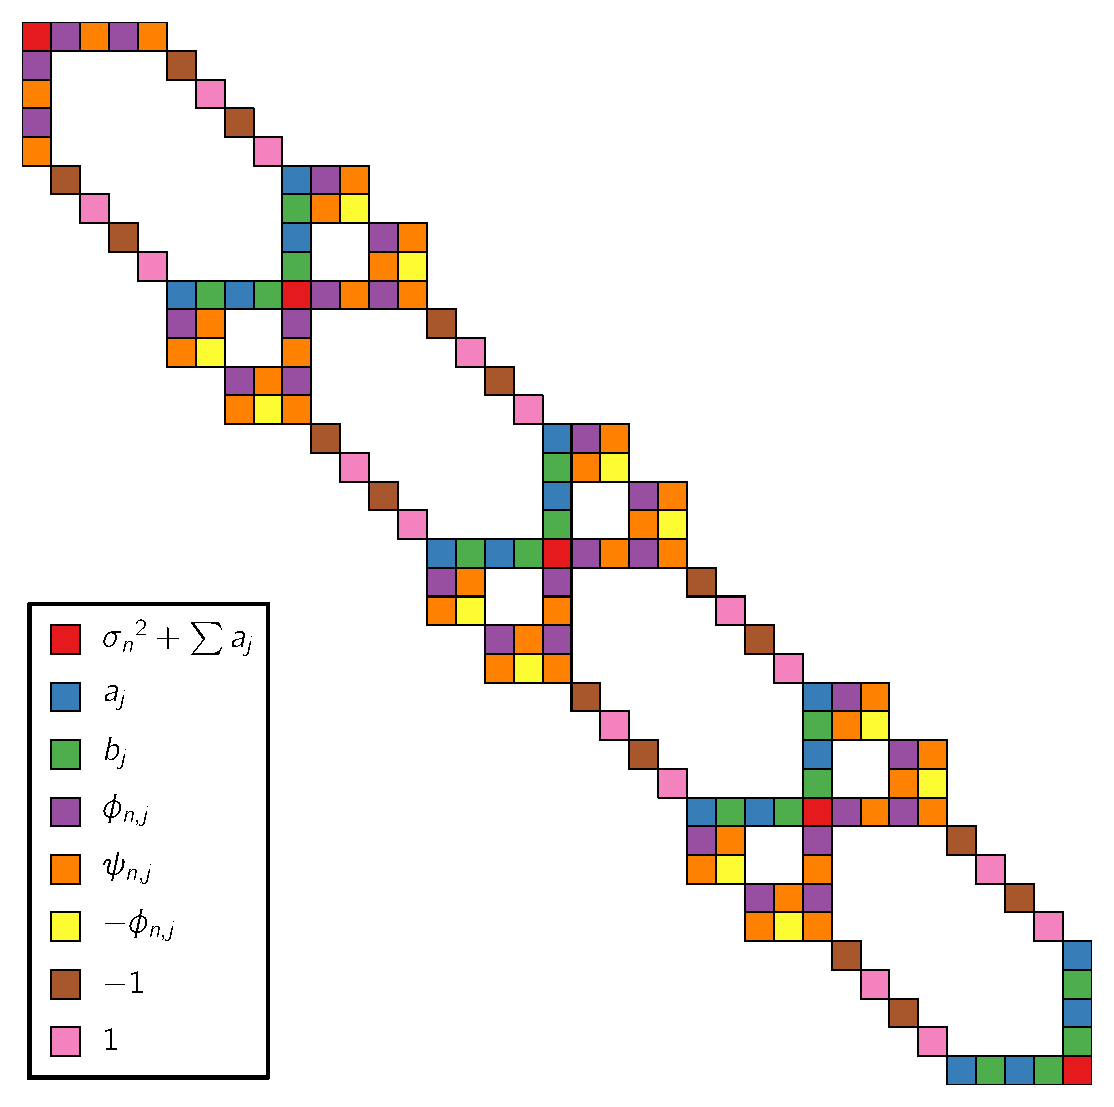
\includegraphics[width=0.7\textwidth]{figures/matrix.pdf}
\caption{A pictorial representation of the sparse extended matrix
$K_\mathrm{ext}$ (\eqalt{kext-full}) with $N=5$ and $J=2$.
Each colored block corresponds to a non-zero entry in the matrix as described
in the legend.
    \figurelabel{matrix}}
\end{center}
\end{figure}

\subsection{Implementation considerations \& scaling}

The extended system defined in the previous section is sparse, with typically
fewer than a few percent non-zero entries and band structure.
In this section, we empirically investigate the performance and scaling
of three different algorithms for solving this extended system:

\begin{enumerate}

\item \texttt{vanilla}: A simple algorithm for computing the LU decomposition
    for banded matrices using Gaussian elimination \citep[we implemented this
    method following][]{Press:1992, Press:2007},

\item \texttt{lapack}: The general banded LU decomposition implementation from
    \project{LAPACK}\footnote{We use the \texttt{dgbtrf} and \texttt{dgbtrs}
    methods from \project{LAPACK}.} \citep{Anderson:1999} using optimized
    \project{BLAS} routines,\footnote{The experiments in this paper use the
    Intel Math Kernel Library (\project{MKL}):
    \url{https://software.intel.com/en-us/intel-mkl}.} and

\item \texttt{sparse}: A general sparse LU solver~--~the \texttt{SparseLU}
    solver from \project{Eigen} \citep{Guennebaud:2010}~--~that exploits the
    sparsity but not the band structure.

\end{enumerate}

The theoretical scaling for a band LU decomposition is $\mathcal{O}(N\,J^3)$
because the dimension of the extended matrix scales as $N\,J$ and the
bandwidth scales with $J$ \citep{Press:1992, Press:2007}.
\citet{Ambikasaran:2015} found an empirical scaling of $\mathcal{O}(N\,J^2)$ that used the sparse LU decomposition implemented in the
\project{SuperLU} package \citep{Demmel:1999}.
We find that, while the \texttt{vanilla} solver scales as expected, the
\texttt{lapack} implementation scales empirically as $\mathcal{O}(N\,J^2)$ and
offers the fastest solves for $J \gtrsim 8$ on all platforms that we tested.

The benchmark experiments shown here were performed on a MacBook Pro with two
2.6~GHz CPUs but we find similar results on a Dell workstation with 16 2.7~GHz
CPUs and running Ubuntu.
\Figure{benchmark} shows how the cost of computing \eq{gp-likelihood} scales
with $N$ and $J$ using the \texttt{vanilla} solver.
As expected theoretically, the scaling is linear in $N$ for all $N$ and cubic
in $J$ for large $J$.
\Figure{benchmark-lapack} and \Figure{benchmark-sparse} are the same plots for
the \texttt{lapack} and \texttt{sparse} solvers respectively.
For each of these optimized solvers, the empirical scaling is
$\mathcal{O}(N\,J^2)$ at the cost of some extra overhead.
Therefore, for $J \lesssim 5$ or $10$ the \texttt{vanilla} solver is more
efficient than the other algorithms.
The real world performance of \celerite\ depends on the specific platform,
hardware, and \project{LAPACK}/\project{BLAS} implementation, but we have
found qualitatively similar results across popular platforms and
state-of-the-art libraries.

\begin{figure}[tp]
\begin{center}
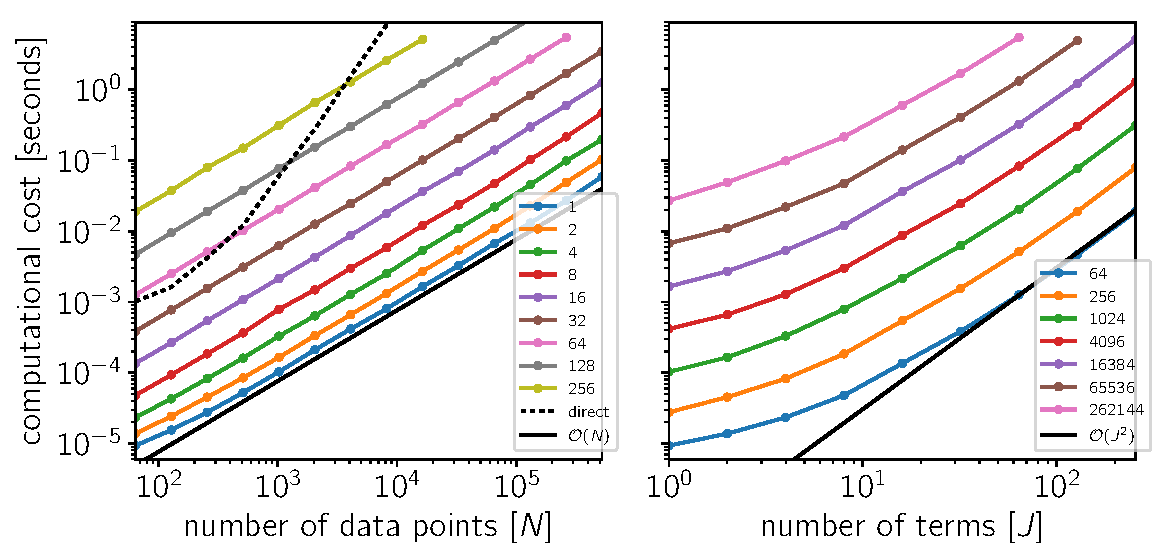
\includegraphics[width=\textwidth]{figures/benchmark_darwin.pdf}
\caption{\dfmtodo{Cholesky} A benchmark showing the computational scaling of \celerite\ using the
    \texttt{vanilla} band solver as a function of the number of data points
    and the number of terms.
    \emph{(left)} The cost of computing \eq{gp-likelihood} with a covariance
    matrix given by \eq{celerite-kernel} as a function of the number of data
    points $N$.
    The different lines show the cost for different numbers of terms $J$
    increasing from bottom to top.
    To guide the eye, the straight black line without points
    shows linear scaling in $N$.
    \emph{(right)} The same information plotted as a function of $J$ for
    different values of $N$.
    Each line shows the scaling for a specific value of $N$ increasing from
    bottom to top.
    The black line shows quadratic scaling in $J$.
    \figurelabel{benchmark}}
\end{center}
\end{figure}


\section{Ensuring positive definiteness}

For a GP kernel to be valid, it must produce a positive definite covariance
matrix for all input coordinates.
For stationary kernels, this is equivalent~--~by Bochner's theorem \citep[see
Section 4.2.1 in][]{Rasmussen:2006}~--~to requiring that the kernel be the
Fourier transform of a positive finite measure.
This means that the power spectrum of a positive definite kernel must be
positive for all frequencies.
This result is intuitive because, since the power spectrum of a process is
defined as the expected squared amplitude of the Fourier transform of the time
series, it must be non-negative.

Using \eq{celerite-psd}, we find that for a single \celeriteterm\ term, this
requirement is met when
\begin{eqnarray}\eqlabel{psd-req}
\frac{(a_j\,c_j+b_j\,d_j)\,({c_j}^2+{d_j}^2)+(a_j\,c_j-b_j\,d_j)\,\omega^2}
{\omega^4+2\,({c_j}^2-{d_j}^2)\,\omega^2+{({c_j}^2+{d_j}^2)}^2} > 0 \quad.
\end{eqnarray}
The denominator is positive for all $c_j \ne 0$ and it can be shown that, when
$c_j=0$, \eq{psd-req} is satisfied for all $\omega \ne d_j$ where the power is
identically zero.
Therefore, when $c_j \ne 0$, we require that the numerator is positive for all
$\omega$.
This requirement can also be written as
\begin{eqnarray}
a_j\,c_j > -b_j\,d_j \\
a_j\,c_j > b_j\,d_j \quad.
\end{eqnarray}
Furthermore, we can see that $a_j$ must be positive since $k(0) = a_j$ should
should be positive and, similarly, by requiring the covariance to be finite at
infinite lag, we obtain the constraint $c_j \ge 0$.
Combining these results, we find the constraint
\begin{eqnarray}
    |b_j\,d_j| < a_j\,c_j \quad.
\end{eqnarray}

In the case of $J$ \celeriteterm\ terms, we can check for negative values of the
PSD by solving for the roots of the power spectrum; if there are any real,
positive roots, then the power-spectrum goes negative (or zero), and thus does not
represent a valid kernel. We rewrite the power spectrum, \eqalt{celerite-psd}),
abbreviating with $z = \omega^2$:
\begin{equation}
S(\omega)=  \sum_{j=1}^J \frac{q_j\,z + r_j}{z^2+s_j\,z + t_j} = 0
\end{equation}
where
\begin{eqnarray}
q_j &=& a_j\,c_j-b_j\,d_j\\
r_j &=& (d_j^2+c_j^2)(b_j\,d_j+a_j\,c_j)\\
s_j &=& 2(c_j^2-d_j^2)\\
t_j &=& (c_j^2+d_j^2)^2.
\end{eqnarray}
The denominators of each term are positive, so we can multiply through by
$\prod_j \left(z^2+s_jz + t_j\right)$ to find
\begin{equation}
Q_0(z) = \sum_{j=1}^J (q_j z + r_j)\prod_{k \ne j}\left(z^2+s_kz +
    t_k\right) = 0\quad,
\end{equation}
which is a polynomial with order $2\,(J-1)+1$.
With $J=2$, this yields a cubic equation whose roots can be obtained exactly.

For arbitrary $J$, a procedure based upon Sturm's theorem \citep{Dorrie:1965}
allows one to determine whether there are any real roots within the range
$(0,\,\infty]$.
We first construct $Q_0(z)$ and its derivative $Q_1(z) = {Q_0}^\prime(z)$,
and then loop from $k=2$ to $k=2\,(J-1)+1$, computing
\begin{eqnarray}
Q_k(z) = -{\rm rem}(Q_{k-2},\,Q_{k-1})
\end{eqnarray}
where the function ${\rm rem}(p,\,q)$ is the remainder polynomial after
dividing $p(z)$ by $q(z)$.

We evaluate the coefficients of each of the polynomial in the series by
evaluating $f_0 = \{Q_0(0),\,\ldots,\,Q_{2\,(J-1)+1}(0)\}$ to give us the signs
of these polynomials evaluated at $z=0$.
Likewise, we evaluate the coefficients of the largest order term in each
polynomial that gives the sign of the polynomial as $z \rightarrow \infty$,
$f_\infty$.
With the sequence of coefficients $f_0$ and $f_\infty$, we then determine how
many times the sign changes in each of these, where $\sigma(0)$ is the number
of sign changes at $z=0$, and $\sigma(\infty)$ is the number of sign changes
at $z \rightarrow \infty$.
The total number of real roots in the range
$(0,\,\infty]$ is given by $N_{+}=\sigma(0)-\sigma(\infty)$.

We have checked that this procedure works for a wide range of parameters, and
we find that it robustly matches the number of positive real roots which we
evaluated numerically.
The advantage of this procedure is that it does not require computing the
roots, but only carrying out algebraic manipulation of polynomials to
determine the number of positive real roots.
If a non-zero real root is found, the likelihood may be set to zero.

\newpage
\bibliography{celerite}

\end{document}
